\part{Capítulo nueve}

\graphicspath{ {9_Capitulo/img/ejemplos/},{9_Capitulo/img/explicacion/}, {W_Varios/2_Portada_capitulos/} }

%----------------------------------------------------------------------------------------
%	CHAPTER 9

\chapter{Valor presente neto}
\section{Mapa Mental}
\begin{center}
	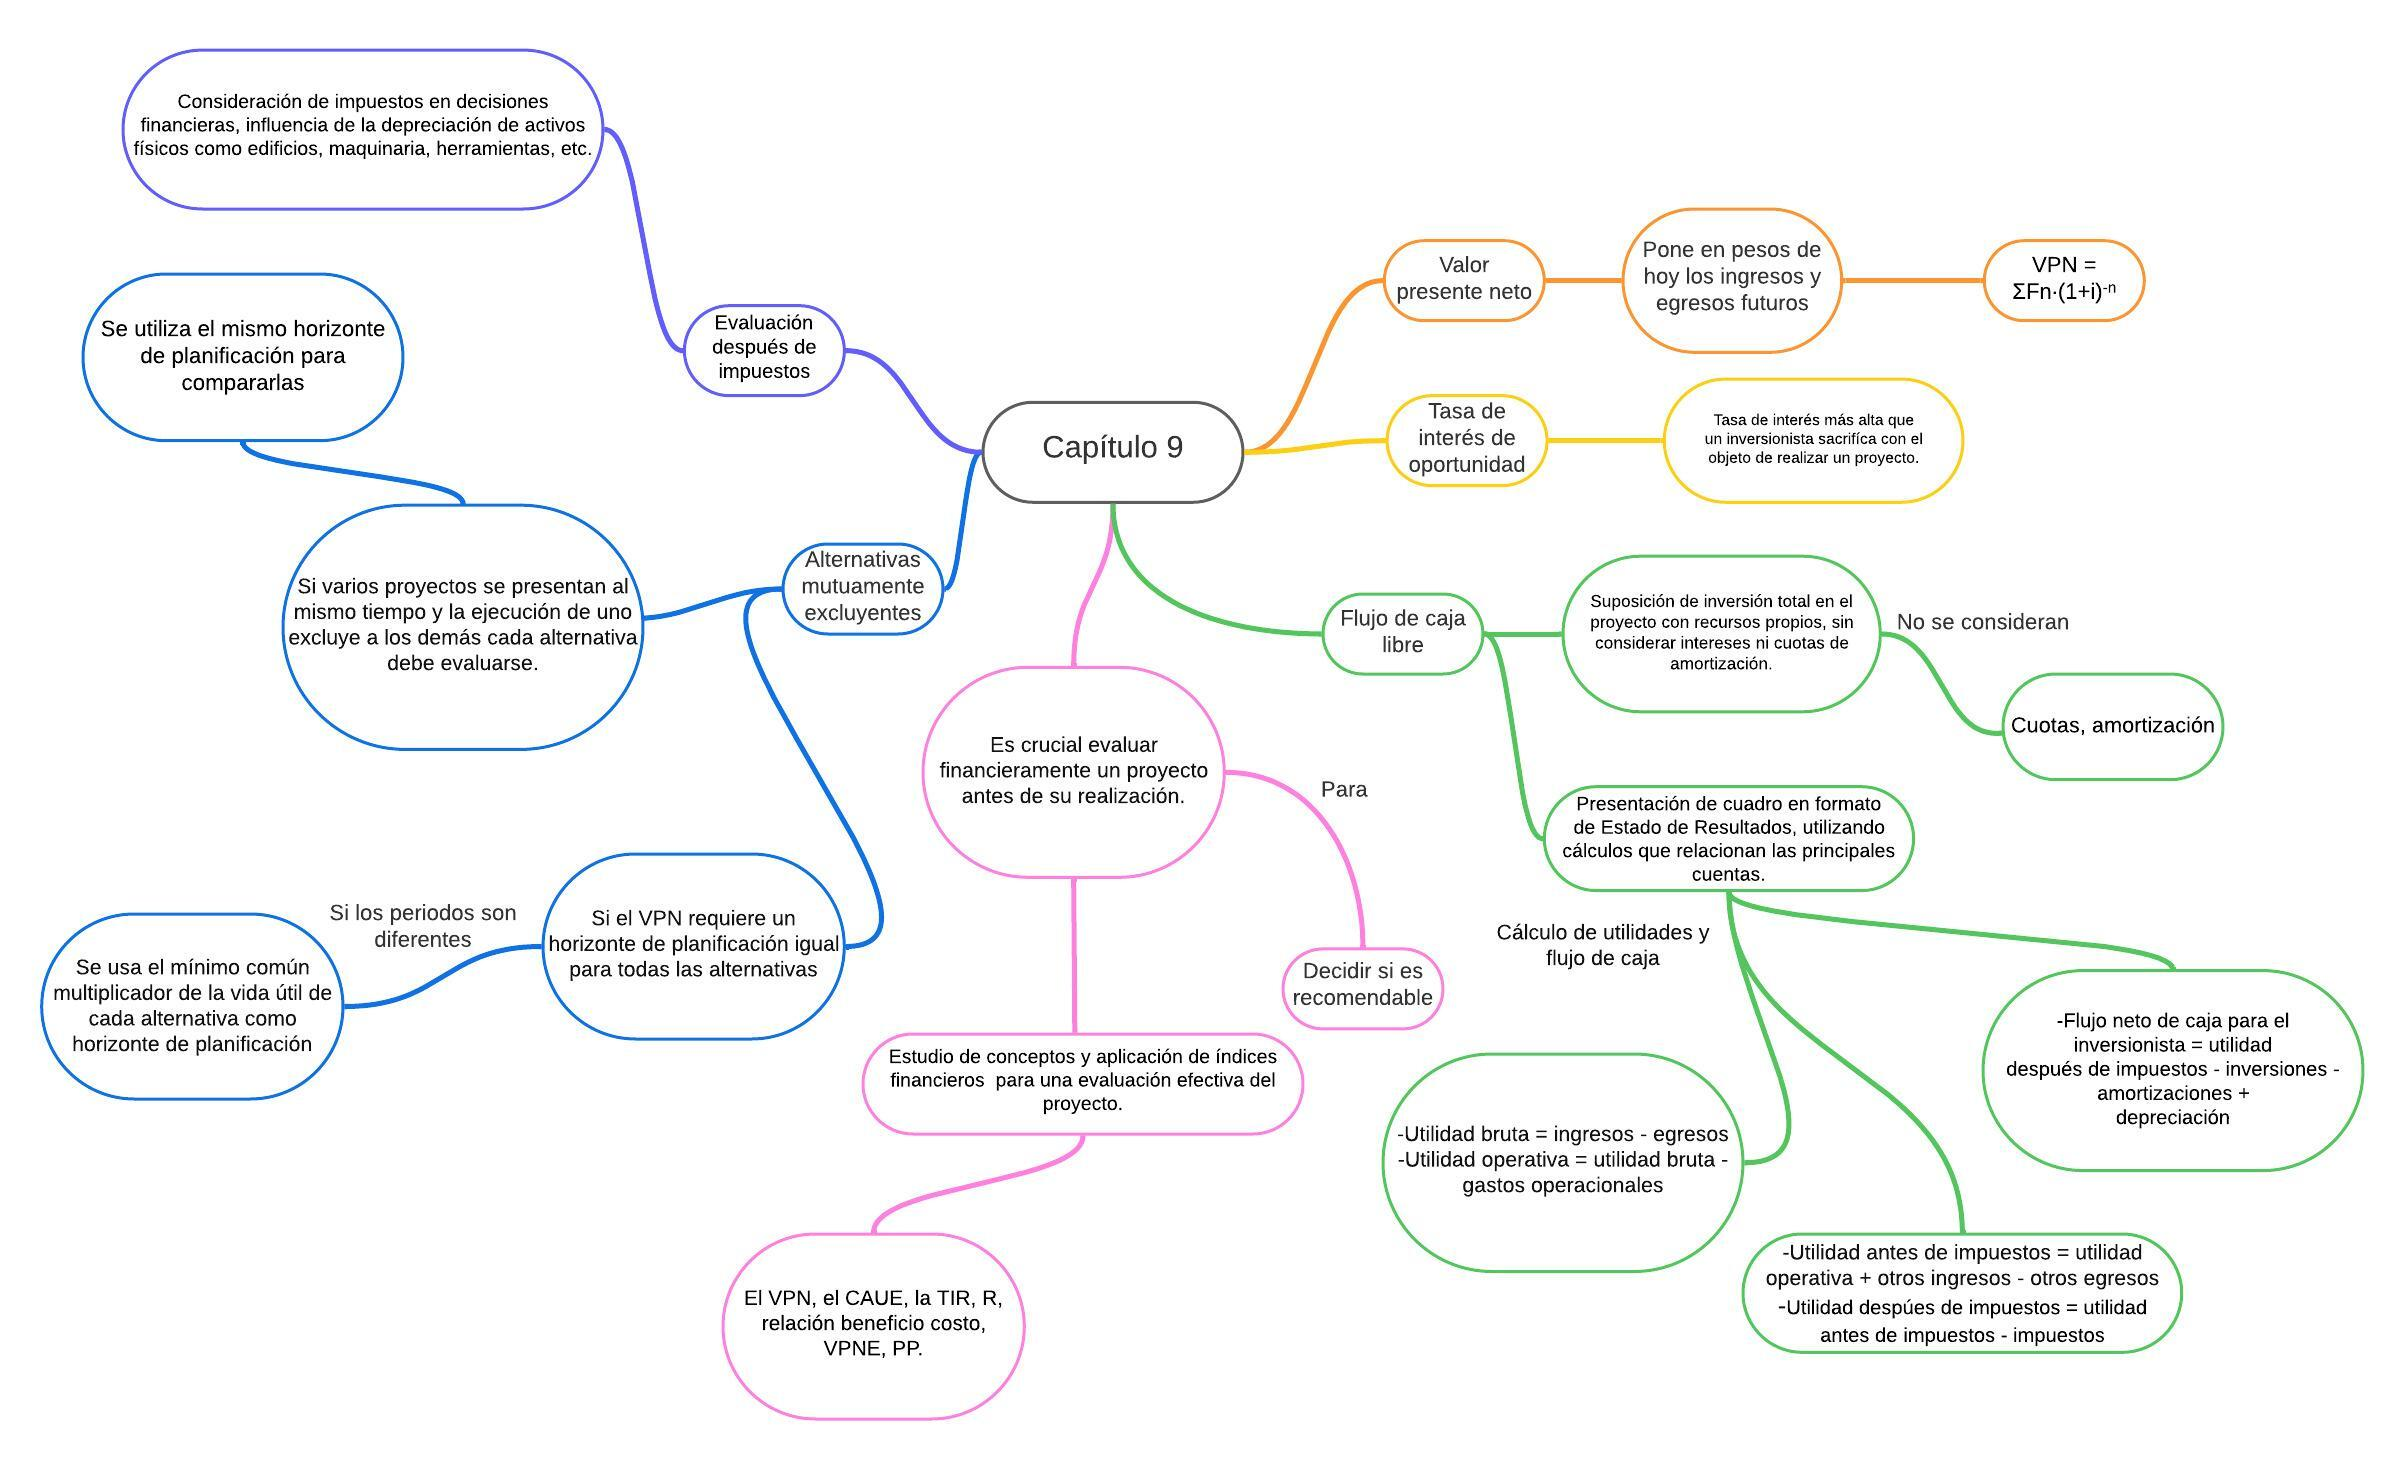
\includegraphics[width=16cm]{9_Capitulo/img/ejemplos/MapMentalCap9.jpeg}
\end{center}
\section{Fórmulas del capítulo}

\begin{spacing}{1.5}
	\begin{center}
		\begin{tabular}{ |p{6cm}|p{5cm}| p{4cm}|}
			\hline
			\rowcolor{orange!50}
			\begin{center}\textbf{Fórmula} \end{center}   & \begin{center} \textbf{Nombre}\end{center} & \begin{center} \textbf{Excel} \end{center} \\ \hline
			
			VPN =	$\sum F_{n}(1+i)^{-n}$ & Valor Presente Neto       & =$SUMPRODUCT(F_n / (1 + i) ^ n)$                         \\ \hline
		\end{tabular}
	\end{center}
\end{spacing}

\section{Introducción}

Es indispensable evaluar un proyecto de inversión financiera antes de llevarlo a cabo, con el objetivo de determinar si es viable y aconsejable. En esta sección, se analizarán conceptos y aplicaciones de indicadores clave, como el Valor Presente Neto (VPN), el Costo Anual Uniforme Equivalente (CAUE), la Tasa Interna de Retorno (TIR), la relación Beneficio-Costo, el Valor Presente Neto Expandido (VPNE), el Período de Payback Ajustado (PPA), entre otros.

\section{VALOR PRESENTE NETO}
El Valor Presente Neto (VPN) es uno de los indicadores más utilizados en la evaluación de proyectos de inversión. Este indicador permite convertir tanto los ingresos como los egresos futuros a pesos actuales, facilitando la toma de decisiones financieras.

\begin{itemize}

\item Si el VPN > 0, el proyecto es rentable, lo que significa que, en términos actuales, los ingresos superan a los egresos.
\item Si el VPN < 0, los ingresos actuales son menores que los egresos, por lo que el proyecto no debería realizarse.
\item Si el VPN = 0, tanto los ingresos como los egresos son equivalentes en términos actuales, haciendo que el proyecto sea  financieramente indiferente para el inversionista.

\end{itemize}

Desde el punto de vista matemático, el VPN se define como la sumatoria de los flujos de caja actualizados al día de hoy, lo que puede representarse mediante la siguiente fórmula:
\begin{center}
	VPN =	$\sum F_{n}(1+i)^{-n}$
\end{center}
\section{Definición de tasa de interés de oportunidad (TIO)}
La Tasa de Interés de Oportunidad (TIO) es la tasa de interés más alta que un inversionista sacrifica con el objetivo de realizar un proyecto. Podemos explicar la definición anterior mediante el siguiente ejemplo: Supongamos que el inversionista ‘A’ tiene las siguientes posibilidades para invertir su dinero:
\begin{enumerate}[label=\alph*)]
	\item Comprar una maquina que le producirá una rentabilidad del 3\% mensual.
	\item Prestar el dinero a un amigo que le pagará con un interés del 2,5 \% mensual.
	\item Invertir en sus negocios normales, los cuales le dan una rentabilidad del 2,8\% mensual.
	\item Invertir en una cuenta de ahorros que paga al 1,5\% mensual.
	\item Invertir en un CDT, donde se le garantiza el 2\% mensual.
\end{enumerate}
El inversionista B solo tiene dos posibilidades:
\begin{enumerate}[label=\alph*)]
	\item Invertir en la cuenta de ahorros con una rentabilidad del 1,5\% mensual.
	\item Invertir en un CDT, donde se le garantiza el 2\% mensual.
\end{enumerate}
De acuerdo con el planteamiento anterior; para el inversionista A, la TIO es del 3\% mensual y para el inversionista B, la TIO será del 2\% mensual.
\\
\\

\textbf{Ejemplo 1}\\
Supongamos que para realizar un proyecto se necesita realizar una inversión inicial de 80.000 COP y otra inversión de 45.000 COP al final del primer mes, en los meses 2 y 3 los ingresos son equivalentes a los egresos pero a partir del mes 4 se producen ingresos así: mes 4 30.000 COP, mes 5 50.000 COP, mes 6 60.000 COP. Determinar si el proyecto lo pueden realizar los inversionistas A o B mencionados anteriormente. Suponga una TIO para el inversionista A del 3\% período mes vencido y para el inversionista B del 2\% período mes vencido.\\



%%%%%%%%%%%%%%%%%%% EJERCICIO 1 %%%%%%

%\newpage %USAR SOLO SI EL SOLUCION QUEDA SOLO Y ES NECESARIO BAJARLO A LA SIGUIENTE PAGINA
\textbf{Solución.}\\
%La tabla ira centrada
\begin{center}
	\renewcommand{\arraystretch}{1.5}% Margenes de las celdas
	%Creacion de la cuadricula de 3 columnas \end{flushleft}
	\begin{longtable}[H]{|C{0.3\linewidth}|C{0.3\linewidth}|C{0.3\linewidth}|}
		%Creamos una linea horizontal
		\hline
         %%%%% INICIO FLUJO DE CAJA
		\rowcolor[HTML]{FFB183}
		\multicolumn{3}{|c|}{\cellcolor[HTML]{FFB183}\textbf{1. Asignación periodo focal}}   \\ \hline
		\multicolumn{3}{|c|} {$pf: 0 pv$} \\ \hline
		%%%%%%%%%% FIN TITULO
		%%%%%%%%%% INICIO TITULO
		%Lo que se hace aqui es mezclar las 3 columnas en una sola
		\multicolumn{3}{|c|}{\cellcolor[HTML]{FFB183}\textbf{2. Declaración de variables}}   \\ \hline
		\multicolumn{1}{|c|}{\cellcolor[HTML]{FFB183}\textbf{Variables monetarias}}                   & \multicolumn{1}{|c|}{\cellcolor[HTML]{FFB183}\textbf{Variables Conceptuales}}                   & \multicolumn{1}{|c|}{\cellcolor[HTML]{FFB183}\textbf{Variables incógnitas}}                                                                         \\ \hline

		%%%%%%%%%% FIN TITULO
		%%%%%%%%%% INICIO DE MATEMATICAS
		%Cada & hace referencia al paso de la siguiente columna

		$P_{0} = -80{.}000COP(P=Egresos)$ & $i_{a} = TIO_{a} = 3\%pmv \equiv 0,03 pmv$ & $VPN_{A}= ? COP$ \\[1em]
		$P_{1} = -45{.}000COP$ & $i_{b} = TIO_{b} = 2\%pmv \equiv 0,02 pmv$ & $VPN_{B}= ? COP$ \\[1em]
		$F_{1} = 30{.}000COP(F=Ingresos)$ & $n_{a} = n_{b} = 6 pmv$ & \\[1em]
		$F_{2} = 50{.}000COP$ & $n_{1} = 1 pmv$ & \\[1em]
		$F_{3} = 60{.}000COP$ & $n_{2} =  4 pmv$ & \\[1em]
		 & $n_{3} = 5 pmv$ & \\[1em]
		 & $n_{4} = 6 pmv$ &
        
        \\\hline

		%%%%%%%%%% FIN DE MATEMATICAS
		%%%%% FIN DECLARACION DE VARIABLES


		%%%%% INICIO FLUJO DE CAJA
		\rowcolor[HTML]{FFB183}
		\multicolumn{3}{|c|}{\cellcolor[HTML]{FFB183}\textbf{3. Diagrama de flujo de caja}} \\ \hline
		%Mezclamos 3 columnas y ponermos el dibujo
		%%%%%%%%%%%%% INSERCION DE LA IMAGEN
		%Deberan descargar las imagenes respectivas del drive y pegarlas en la carpeta
		%n_capitulo/img/ejemplos/1/capitulo1ejemplo1.pdf  (el /1/ es el numero del ejemplo)
		\multicolumn{3}{|c|}{ 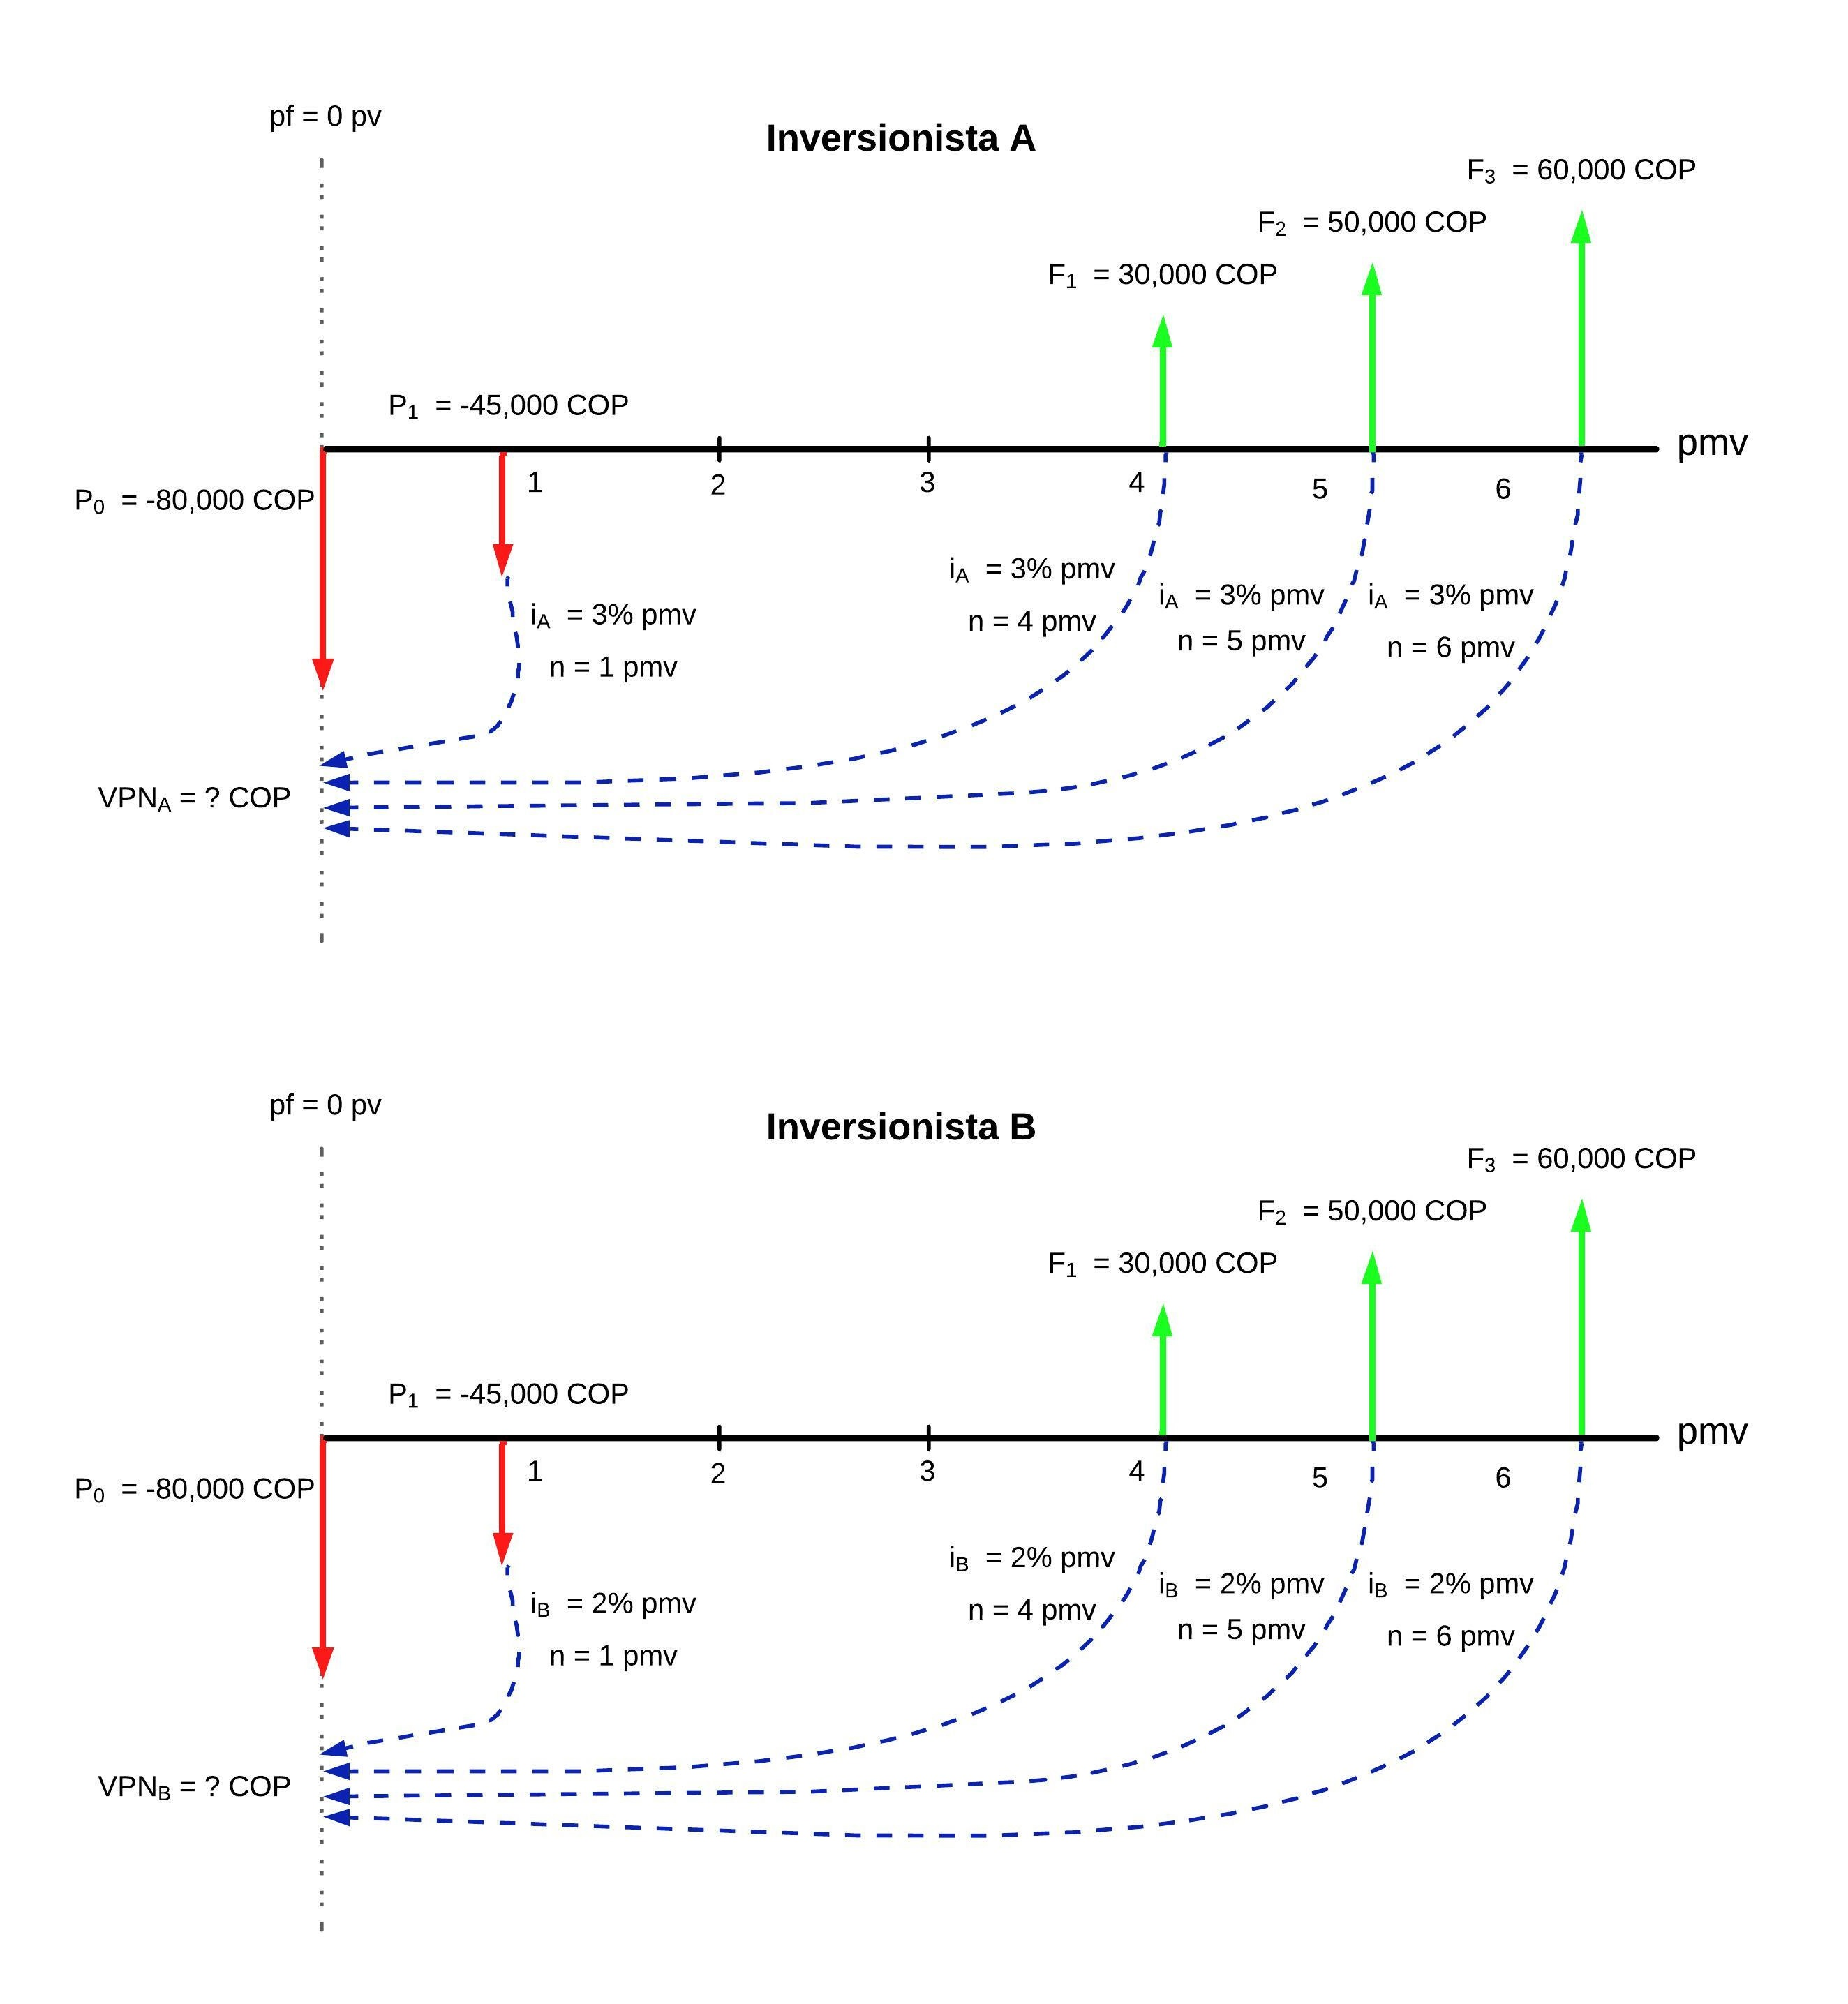
\includegraphics[trim=-5 -5 -5 -5 , scale=1,width=380px, height=450px]{9_Capitulo/ejemplos/1/exportados/DiaCEjem1Cap9(1).png} }   \\ \hline
		%%%%%%%%%%%%% FIN INSERCION DE IMAGEN
		%%%%%FIN FLUJO DE CAJA



		%%%%% INICIO DECLARACION FORMULAS
		%%%%%%%%%%% INICIO TITULO
		\rowcolor[HTML]{FFB183}
		\multicolumn{3}{|c|}{\cellcolor[HTML]{FFB183}\textbf{4. Declaración de fórmulas}}    \\ \hline
		%%%%%%%%%%% FIN TITULO
		%%%%%%%%%%% INICIO MATEMATICAS
		\multicolumn{3}{|c|}{$\sum F_{n}(1+i)^{-n} $\hspace{0.3cm} \textit{Valor presente neto}} \\ \hline
		%%%%%%%%%% FIN MATEMATICAS
		%%%%%% INICIO DESARROLLO MATEMATICO
		\rowcolor[HTML]{FFB183}
		%%%%%%%%%%INICIO TITULO
		\multicolumn{3}{|c|}{\cellcolor[HTML]{FFB183}\textbf{5. Desarrollo matemático}}       \\ \hline
		%%%%%%%%%% FIN TITULO
		%%%%%%%%%% INICIO MATEMATICAS
		\multicolumn{3}{|c|}{$VPN_{a} = -80{.}000COP(1+0pmv)^{-0pmv} - 45{.}000COP(1+0.03pmv)^{-1pmv} $} \\
        \multicolumn{3}{|l|}{$+ 30{.}000COP(1+0.03pmv)^{-4pmv} + 50{.}000COP(1+0.03pmv)^{-5pmv} + 60{.}000COP(1+0.03pmv)^{-6pmv}$}
        \\
		\multicolumn{3}{|c|}{$VPN_{a} = -3{.}655COP$} \\
		\multicolumn{3}{|c|}{$VPN_{b} = -80{.}000COP(1+0pmv)^{0pmv} - 45{.}000COP(1+0.02pmv)^{-1pmv}$} \\
        \multicolumn{3}{|l|}{$+ 30{.}000COP(1+0.02pmv)^{-4pmv} + 50{.}000COP(1+0.02pmv)^{-5pmv} + 60{.}000COP(1+0.02pmv)^{-6pmv}$} \\ \multicolumn{3}{|c|}{$VPN_{b} = 2{.}162COP$} \\ \hline

		%%%%%%%%%% FIN MATEMATICAS
		%%%%%% FIN DESARROLLO MATEMATICO
		%%%%%% INICIO RESPUESTA
		\rowcolor[HTML]{FFB183}
		%%%%%%%%%%INICIO TITULO
		\multicolumn{3}{|c|}{\cellcolor[HTML]{FFB183}\textbf{6. Respuesta}}   \\ \hline
		%%%%%%%%%% FIN TITULO
		%%%%%%%%%% INICIO RESPUESTA MATEMATICA
        \multicolumn{3}{|c|}{En un proyecto llevado a cabo por dos inversionistas A y B, se tiene:}  \\
        \multicolumn{3}{|c|}{Para el inversionista A, VPN < 0, es decir que, no se recomienda realizar el proyecto} \\
        \multicolumn{3}{|c|}{Para el inversionista B, VPN > 0, es decir que, se recomienda realizar el proyecto} \\ \hline

		%%%%%%%%%% FIN MATEMATICAS
		%%%%%% FIN RESPUESTA
	\end{longtable}
	%Se crean dos lineas en blanco para que no quede el siguiente texto tan pegado
	%\newline \newline %USARLO SI CREES QUE ES NECESARIO
\end{center}
%%%%%%%%%%%%%%%%%%%%%%%%%%FIN EJERCICIO 1 %%%%%%%%%%%%%%%%%%%%%%%%%%%


\section{Símbolos.}

Con el fin de facilitar la construcción de gráficas y, para simplificar la escritura, adoptaremos los siguientes símbolos.\\

$C_{0}$  =  Costo inicial o inversión inicial.\\
$C_{1}$ =  Costos en el período 1 o inversión en el periodo 1.\\
$C_{2}$  =  Costos en el período 2 o inversión en el periodo 2.\\
.\\
.\\
.\\
Cn  =  Costo en el período n o inversión en el periodo n.\\
K  =  Vida útil (expresada en años, en meses o en unidades producidas).\\
S  =  Valor de salvamento.\\
CAO  =  Costo anual de operación o serie neta uniforme de costo de operación, cuando los costos son mensuales se representará por CMO.\\
$I_{1}$  =  Ingreso en el período 1.\\
$I_{2}$  =  Ingreso en el período 2.\\
.\\
.\\
.\\
In  =  Ingreso del período n.\\

\section{UTILIZACIÓN DEL VPN}

El VPN puede utilizarse tanto en proyectos individuales como en la decisión sobre alternativas de inversión. En el primer caso, basta con conocer el signo del VPN para tomar una decisión, como se puede apreciar en el siguiente ejemplo:\\
\\
\textbf{Ejemplo 2}\\
Un proyecto requiere de una inversión inicial de 100.000 COP y se cree que generará unos ingresos de 65.000 COP al final del primer año y de 75.000 COP al final del segundo año. Evaluar el proyecto para el inversionista A cuya tasa es del 20\% período año vencido, y para el inversionista B cuya tasa es del 40\% período año vencido.\\


%%%%%%%%%%%%%%%%%%% EJERCICIO 2 %%%%%%

%\newpage %USAR SOLO SI EL SOLUCION QUEDA SOLO Y ES NECESARIO BAJARLO A LA SIGUIENTE PAGINA
\textbf{Solución.}\\
%La tabla ira centrada
\begin{center}
	\renewcommand{\arraystretch}{1.5}% Margenes de las celdas
	%Creacion de la cuadricula de 3 columnas \end{flushleft}
	\begin{longtable}[H]{|C{0.3\linewidth}|C{0.3\linewidth}|C{0.3\linewidth}|}
		%Creamos una linea horizontal
		\hline
        %%%%% INICIO FLUJO DE CAJA
		\rowcolor[HTML]{FFB183}
		\multicolumn{3}{|c|}{\cellcolor[HTML]{FFB183}\textbf{1. Asignación periodo focal}}   \\ \hline
		\multicolumn{3}{|c|} {$pf: 0pv$} \\ \hline
		%%%%%%%%%% FIN TITULO
		%%%%%%%%%% INICIO TITULO
		%Lo que se hace aqui es mezclar las 3 columnas en una sola
		\multicolumn{3}{|c|}{\cellcolor[HTML]{FFB183}\textbf{2. Declaración de variables}}   \\ \hline
		\multicolumn{1}{|c|}{\cellcolor[HTML]{FFB183}\textbf{Variables monetarias}}                   & \multicolumn{1}{|c|}{\cellcolor[HTML]{FFB183}\textbf{Variables Conceptuales}}                   & \multicolumn{1}{|c|}{\cellcolor[HTML]{FFB183}\textbf{Variables incógnitas}}                                                                         \\ \hline

		%%%%%%%%%% FIN TITULO
		%%%%%%%%%% INICIO DE MATEMATICAS
		%Cada & hace referencia al paso de la siguiente columna

		$P_{0} = -100{.}000COP(P=Egresos)$ & $i_{A} = TIO_{A} = 20\% pav \equiv 0.2 pav$ & $VPN_{A}= ? COP$ \\ [1em]
		$F_{1} = 65{.}000COP(F=Ingresos)$ & $i_{B} = TIO_{B} = 40\% pav \equiv 0.4 pav$ & $VPN_{B}= ? COP$ \\ [1em]
		$F_{2} = 75{.}000COP$ & $n_{a} = n_{b} = 6 pmv$ & \\ [1em]
		& $n_{0} = 0 pav$ & \\[1em]
		& $n_{1} = 1 pav$ & \\[1em]
		& $n_{2} =  2pav$ & \\

        \hline
		%%%%%%%%%% FIN DE MATEMATICAS
		%%%%% FIN DECLARACION DE VARIABLES


  	%%%%% INICIO DECLARACION FORMULAS
  
		%%%%%%%%%%% INICIO TITULO
		\rowcolor[HTML]{FFB183}
		\multicolumn{3}{|c|}{\cellcolor[HTML]{FFB183}\textbf{3. Diagrama de flujo de caja}} \\ \hline
		%Mezclamos 3 columnas y ponermos el dibujo
		%%%%%%%%%%%%% INSERCION DE LA IMAGEN
		%Deberan descargar las imagenes respectivas del drive y pegarlas en la carpeta
		%n_capitulo/img/ejemplos/1/capitulo1ejemplo1.pdf  (el /1/ es el numero del ejemplo)
		\multicolumn{3}{|c|}{ 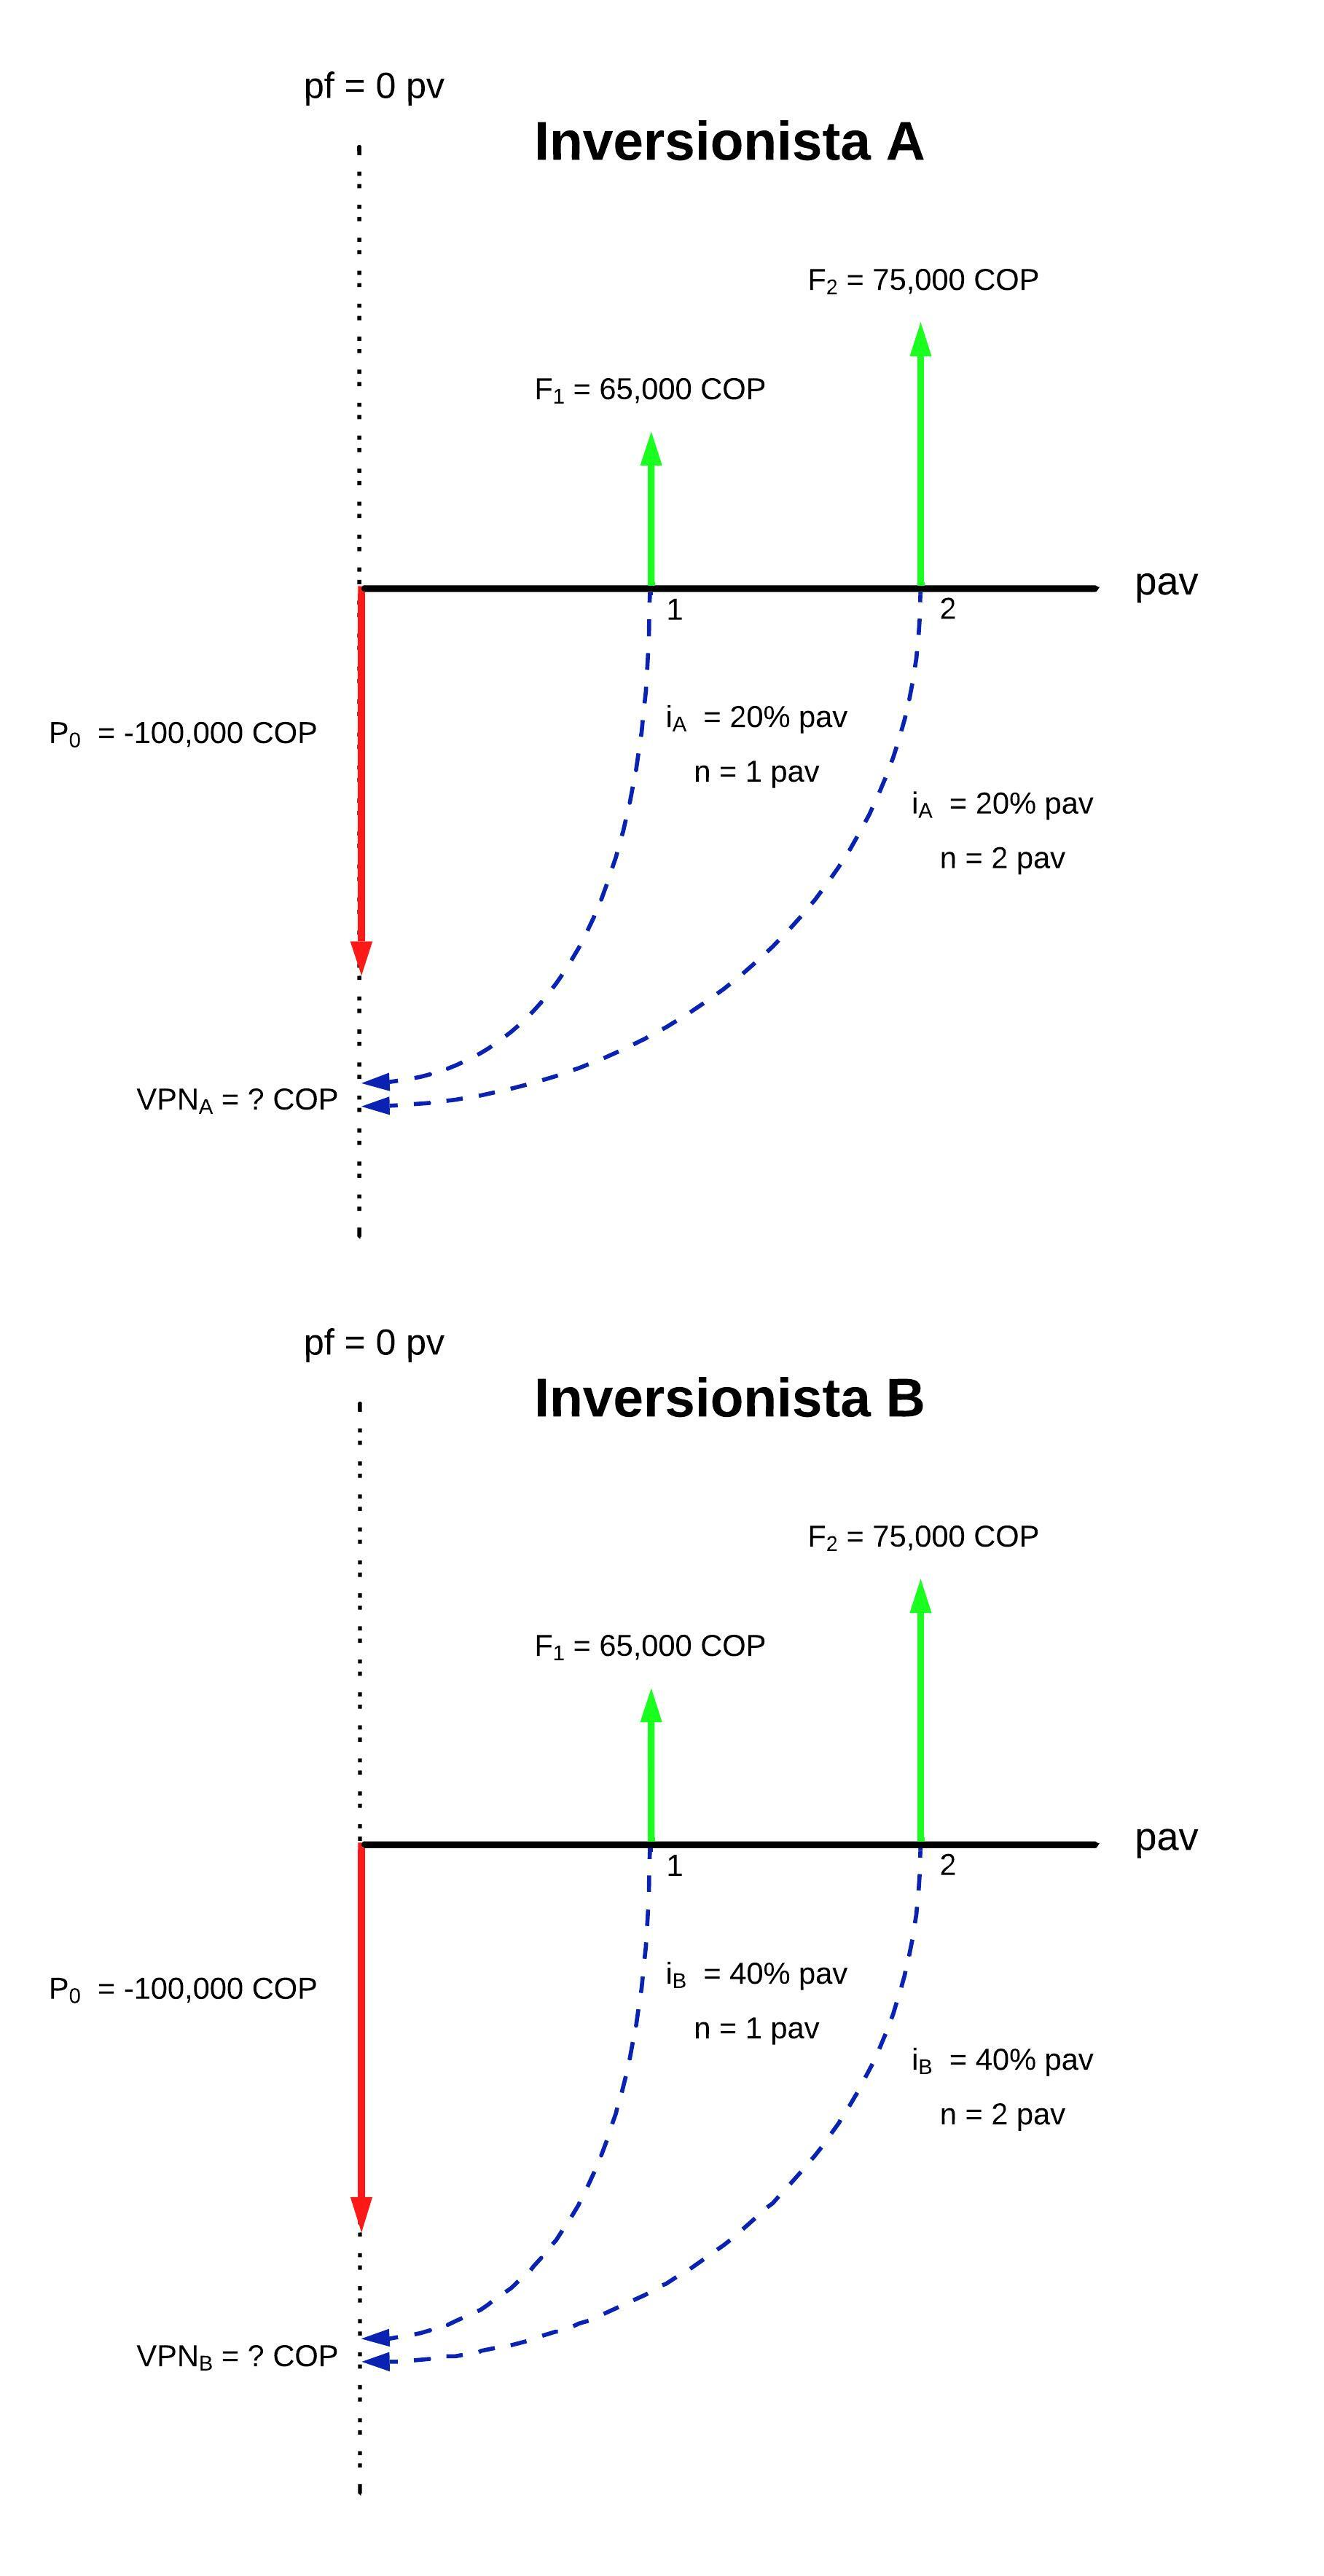
\includegraphics[trim=-5 -5 -5 -5 , scale=1, width=245px, height=425px]{9_Capitulo/ejemplos/2/exportados/DiaCEjem2Cap9(1).png} }   \\ \hline
		%%%%%%%%%%%%% FIN INSERCION DE IMAGEN
		%%%%%FIN FLUJO DE CAJA



		%%%%% INICIO DECLARACION FORMULAS
		%%%%%%%%%%% INICIO TITULO
		\rowcolor[HTML]{FFB183}
		\multicolumn{3}{|c|}{\cellcolor[HTML]{FFB183}\textbf{4. Declaración de fórmulas}}    \\ \hline
		%%%%%%%%%%% FIN TITULO
		%%%%%%%%%%% INICIO MATEMATICAS
		\multicolumn{3}{|c|}{$\sum F_{n}(1+i)^{-n} $\hspace{0.3cm} \textit{Valor presente neto}} \\ \hline
		%%%%%%%%%% FIN MATEMATICAS
		%%%%%% INICIO DESARROLLO MATEMATICO
		\rowcolor[HTML]{FFB183}
		%%%%%%%%%%INICIO TITULO
		\multicolumn{3}{|c|}{\cellcolor[HTML]{FFB183}\textbf{5. Desarrollo matemático}}       \\ \hline
		%%%%%%%%%% FIN TITULO
		%%%%%%%%%% INICIO MATEMATICAS
		\multicolumn{3}{|c|}{$VPN_{A} = -100{.}000COP(1+0pav)^{0pav}  + 65{.}000COP(1+0,2pav)^{-1pav} + 75{.}000COP(1+0,2pav)^{-2pav}$} \\
		\multicolumn{3}{|c|}{$VPN_{A} = 6{.}250COP$} \\
		\multicolumn{3}{|c|}{$VPN_{B} = -100{.}000COP(1+0pav)^{0pav}  + 65{.}000COP(1+0,4pav)^{-1pav} + 75{.}000COP(1+0,4pav)^{-2pav}$} \\
		\multicolumn{3}{|c|}{$VPN_{B} = -15{.}506COP$} \\ \hline

		%%%%%%%%%% FIN MATEMATICAS
		%%%%%% FIN DESARROLLO MATEMATICO
		%%%%%% INICIO RESPUESTA
		\rowcolor[HTML]{FFB183}
		%%%%%%%%%%INICIO TITULO
		\multicolumn{3}{|c|}{\cellcolor[HTML]{FFB183}\textbf{6. Respuesta}}   \\ \hline
		%%%%%%%%%% FIN TITULO
		%%%%%%%%%% INICIO RESPUESTA MATEMATICA

        \multicolumn{3}{|c|}{Para el inversionista A, VPN > 0, es decir que, se recomienda realizar el proyecto}\\
        \multicolumn{3}{|c|}{Para el inversionista B, VPN < 0, es decir que, no se recomienda realizar el proyecto} \\ \hline

		%%%%%%%%%% FIN MATEMATICAS
		%%%%%% FIN RESPUESTA
	\end{longtable}
	%Se crean dos lineas en blanco para que no quede el siguiente texto tan pegado
	%\newline \newline %USARLO SI CREES QUE ES NECESARIO
\end{center}
%%%%%%%%%%%%%%%%%%%%%%%%%%FIN EJERCICIO 2 %%%%%%%%%%%%%%%%%%%%%%%%%%%


\section{ALTERNATIVAS MUTUAMENTE EXCLUYENTES}

Puede ocurrir que simultáneamente se presenten varios proyectos, pera la ejecución de uno de ellos excluye la posibilidad de ejecución de cualquiera de los otros, en este caso se debe evaluar cada alternativa por separado, pero siempre usando el mismo horizonte de planeación a fin de poderlos comparar.\\
\\
\textbf{Ejemplo 3}\\
Una fabrica produce actualmente en forma manual 1.000 unidades de un determinado artículo, para ello utiliza artesanos a los cuales les paga 8.400.000 COP al año y, es costumbre que cada año se les aumente el sueldo en aproximadamente un 20\% período año vencido. El precio de venta de cada artículo es de 9.000 COP y se estima que este precio podrá ser aumentado todos los años en un 21\% período año vencido. Ahora se ha presentado la oportunidad de adquirir una máquina a un costo de 10 millones COP con una vida útil de 5 años; un valor de salvamento de 2 millones COP la cual requiere de 2 técnicos para su operación, el sueldo anual de cada uno de los técnicos puede ser de 600.000 COP con aumentos anuales de sueldo del 20\% período año vencido ¿Cuál de las dos alternativas es mejor suponiendo que la tasa del inversionista es del 30\% período año vencido?\\


%%%%%%%%%%%%%%%%%%% EJERCICIO 3 %%%%%%

%\newpage %USAR SOLO SI EL SOLUCION QUEDA SOLO Y ES NECESARIO BAJARLO A LA SIGUIENTE PAGINA
\textbf{Solución.}\\
%La tabla ira centrada
\begin{center}
	\renewcommand{\arraystretch}{1.5}% Margenes de las celdas
	%Creacion de la cuadricula de 3 columnas \end{flushleft}
	\begin{longtable}[H]{|C{0.3\linewidth}|C{0.3\linewidth}|C{0.3\linewidth}|}
		%Creamos una linea horizontal
		\hline
        %%%%% INICIO FLUJO DE CAJA
		\rowcolor[HTML]{FFB183}
		\multicolumn{3}{|c|}{\cellcolor[HTML]{FFB183}\textbf{1. Asignación periodo focal}}   \\ \hline
		\multicolumn{3}{|c|} {$pf: 0 pav$} \\ \hline
		%%%%%%%%%% FIN TITULO
		%%%%%%%%%% INICIO TITULO
		%Lo que se hace aqui es mezclar las 3 columnas en una sola
		\multicolumn{3}{|c|}{\cellcolor[HTML]{FFB183}\textbf{2. Declaración de variables}}   \\ \hline
		\multicolumn{1}{|c|}{\cellcolor[HTML]{FFB183}\textbf{Variables monetarias}}                   & \multicolumn{1}{|c|}{\cellcolor[HTML]{FFB183}\textbf{Variables Conceptuales}}                   & \multicolumn{1}{|c|}{\cellcolor[HTML]{FFB183}\textbf{Variables incógnitas}}                                                                         \\ \hline

		%%%%%%%%%% FIN TITULO
		%%%%%%%%%% INICIO DE MATEMATICAS
		%Cada & hace referencia al paso de la siguiente columna
		$F_{1} = 9{.}000{.}000 $ COP & $i_{1} =  21\% pav $ & Decisión final.\\[1em]
		$F_{2} = 8{.}400{.}000$ COP & $n_{1} =  5 pav $ & \\[1em]
		& $i_{2}=  20\% pav $ & \\[1em]
		& $n_{2}= 5 pav$ & \\[1em]
		& $i_{3}=30\% pav$ & \\[1em]
		& $n=5pav$ &
  
		\\\hline
		%%%%%%%%%% FIN DE MATEMATICAS
		%%%%% FIN DECLARACION DE VARIABLES

  		%%%%% INICIO DECLARACION FORMULAS
  
		%%%%%%%%%%% INICIO TITULO
		\rowcolor[HTML]{FFB183}
		\multicolumn{3}{|c|}{\cellcolor[HTML]{FFB183}\textbf{3. Diagrama de flujo de caja}} \\ \hline
		%Mezclamos 3 columnas y ponermos el dibujo
		%%%%%%%%%%%%% INSERCION DE LA IMAGEN
		%Deberan descargar las imagenes respectivas del drive y pegarlas en la carpeta
		%n_capitulo/img/ejemplos/1/capitulo1ejemplo1.pdf  (el /1/ es el numero del ejemplo)
		\multicolumn{3}{|c|}{ 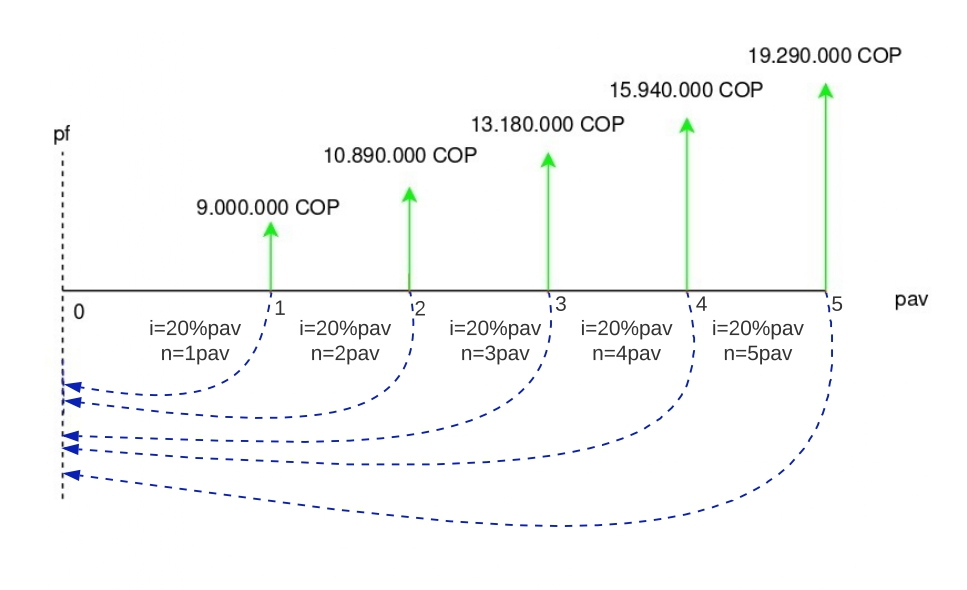
\includegraphics[trim=-5 -5 -5 -5 , scale=1, width=300px, height=250px]{9_Capitulo/ejemplos/3/exportados/ejercicio 3a.png} }   \\ 
   \multicolumn{3}{|c|}{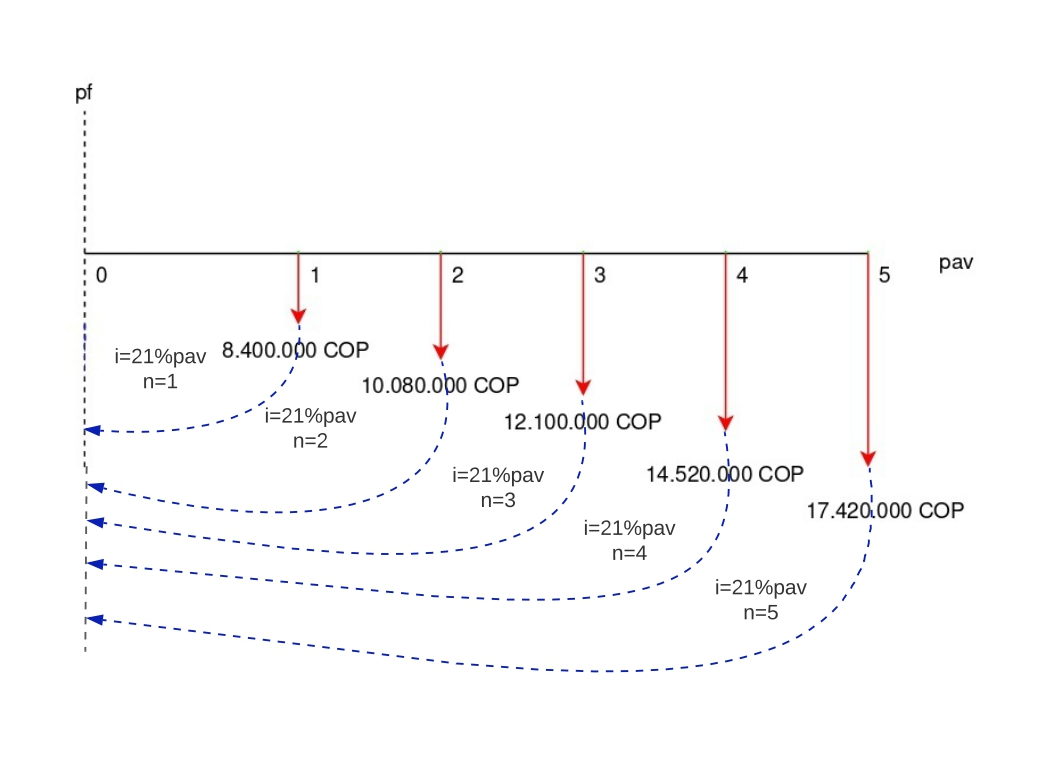
\includegraphics[trim=-5 -5 -5 -5 , scale=1,width=300px, height=250px]{9_Capitulo/ejemplos/3/exportados/ejercicio 3b.png} } \\
         \hline
		%%%%%%%%%%%%% FIN INSERCION DE IMAGEN
		%%%%%FIN FLUJO DE CAJA



		%%%%% INICIO DECLARACION FORMULAS
		%%%%%%%%%%% INICIO TITULO
		\rowcolor[HTML]{FFB183}
		\multicolumn{3}{|c|}{\cellcolor[HTML]{FFB183}\textbf{4. Declaración de fórmulas}}    \\ \hline
		%%%%%%%%%%% FIN TITULO
		%%%%%%%%%%% INICIO MATEMATICAS
		\multicolumn{3}{|c|}{$\sum F_{n}(1+i)^{-n} $\hspace{0.3cm} \textit{Valor presente neto}} \\ \hline
		%%%%%%%%%% FIN MATEMATICAS
		%%%%%% INICIO DESARROLLO MATEMATICO
		\rowcolor[HTML]{FFB183}
		%%%%%%%%%%INICIO TITULO
		\multicolumn{3}{|c|}{\cellcolor[HTML]{FFB183}\textbf{5. Desarrollo matemático}}       \\ \hline
		%%%%%%%%%% FIN TITULO
		%%%%%%%%%% INICIO MATEMATICAS
		\multicolumn{3}{|c|}{$VPN_{A} = \frac{9[(1+0.21)^{5}(1+0.3)^{-5} -1]}{0.21-0.3} - \frac{8.4[(1+0.2)^{5}(1+0.3^{-5} -1)]}{0.2-0.3}$} \\
		\multicolumn{3}{|c|}{$VPN_{A} = 2{.}437{.}836 $ COP} \\
		\multicolumn{3}{|c|}{$VPN_{B} = \frac{9[(1+0.21)^{5}(1+0.3)^{-5} -1]}{0.21-0.3} + 2(1.3)^{-5} - \frac{1.2[(1+0.2)^{5}(1+0.3^{-5} -1)]}{0.2-0.3}$} \\
		\multicolumn{3}{|c|}{$VPN_{B} = 16{.}723{.}756 $ COP} \\ \hline

		%%%%%%%%%% FIN MATEMATICAS
		%%%%%% FIN DESARROLLO MATEMATICO
		%%%%%% INICIO RESPUESTA
		\rowcolor[HTML]{FFB183}
		%%%%%%%%%%INICIO TITULO
		\multicolumn{3}{|c|}{\cellcolor[HTML]{FFB183}\textbf{6. Respuesta}}   \\ \hline
		%%%%%%%%%% FIN TITULO
		%%%%%%%%%% INICIO RESPUESTA MATEMATICA
		\multicolumn{3}{|c|}{La decisión correcta es comprar la máquina.}  \\ \hline
		%%%%%%%%%% FIN MATEMATICAS
		%%%%%% FIN RESPUESTA
	\end{longtable}
	%Se crean dos lineas en blanco para que no quede el siguiente texto tan pegado
	%\newline \newline %USARLO SI CREES QUE ES NECESARIO
\end{center}
%%%%%%%%%%%%%%%%%%%%%%%%%%FIN EJERCICIO 3 %%%%%%%%%%%%%%%%%%%%%%%%%%%


\section{ALTERNATIVAS MUTUAMENTE EXCLUYENTES CON DIFERENTE VIDA ÚTIL}

Dado que el VPN exige que el horizonte planeación sea de igual número de períodos en cada alternativa y, en éste caso cada alternativa tiene diferente numero de períodos; entonces es necesario, tomar un horizonte de planeación que sea igual al mínimo común múltiplo de la vida útil de cada una de las alternativas.\\
\\
\textbf{Ejemplo 4}\\
El jefe de producción de una fabrica debe decidir entre el motor A y el motor B, con una tasa del 36\% pav; determinar la mejor alternativa.\\

Las características de cada uno son:

%\begin{spacing}{1.5}
\begin{center}
	\begin{tabular}{ |p{4cm}|p{4cm}| p{4cm}|}
		\hline
		\begin{center}\textbf{-} \end{center} & \begin{center} \textbf{Motor A}\end{center} & \begin{center} \textbf{Motor B} \end{center} \\ \hline
		C (P)                         & 800.000 COP                 & 600.000 COP                  \\ \hline
		K                          & 3                          & 2                          		\\  \hline
		S(F)                          & 200.000 COP                  & 150.000 COP                 \\ \hline
		CAO                        & 25.000 COP                   & 30.000 COP                   \\ \hline
	\end{tabular}
\end{center}
El mínimo común múltiplo de la vida útil de las dos alternativas es 6 años, así que el horizonte de planeación será de 6 años.\\
Para la alternativa I, tendríamos después de 3 años tener que adquirir otra maquina de las mismas características y, en la alternativa II, tendríamos que adquirir 3 maquinas; la primera el día de hoy, la segunda a los 2 años y la tercera al final de 4 años:
\\


%%%%%%%%%%%%%%%%%%% EJERCICIO 4 %%%%%%

%\newpage %USAR SOLO SI EL SOLUCION QUEDA SOLO Y ES NECESARIO BAJARLO A LA SIGUIENTE PAGINA
\textbf{Solución.}\\
%La tabla ira centrada
\begin{center}
	\renewcommand{\arraystretch}{1.5}% Margenes de las celdas
	%Creacion de la cuadricula de 3 columnas \end{flushleft}
	\begin{longtable}[H]{|C{0.3\linewidth}|C{0.3\linewidth}|C{0.3\linewidth}|}
		%Creamos una linea horizontal
		\hline
        %%%%% INICIO FLUJO DE CAJA
		\rowcolor[HTML]{FFB183}
		\multicolumn{3}{|c|}{\cellcolor[HTML]{FFB183}\textbf{1. Asignación periodo focal}}   \\ \hline
		\multicolumn{3}{|c|} {$pf : 0 \hspace{0.5em} pav$} \\ \hline
		%%%%%%%%%% FIN TITULO
		%%%%%%%%%% INICIO TITULO
		%Lo que se hace aqui es mezclar las 3 columnas en una sola
		\multicolumn{3}{|c|}{\cellcolor[HTML]{FFB183}\textbf{2. Declaración de variables}}   \\ \hline
		%%%%%%%%%% FIN TITULO
		%%%%%%%%%% INICIO DE MATEMATICAS
		% Cada & hace referencia al paso de la siguiente columna
		$F_{A} =$ 200.000 COP & $K_{A} = 3$ &Decisión final\\ 
		$F_{B} =$ 150.000 COP & $K_{B} = 2$ \\ 
		$P_{A} = $ 800.000 COP & $n_{A} = 6 \hspace{0.5em} pav$\\ 
		$P_{B} = $ 600.000 COP & $n_{B} = 6 \hspace{0.5em} pav$\\ 
		$CAO_{A} = $ 25.000 COP & $i_{A} = 36\% \hspace{0.5em} pav \equiv 0,36 \hspace{0.5em} pav$  \\ 
		$CAO_{B} = $ 30.000 COP & $i_{B} = 36\% pav \hspace{0.5em} \equiv 0,36 \hspace{0.5em} pav$ \\ 

		%%%%%%%%%% FIN DE MATEMATICAS
		%%%%% FIN DECLARACION DE VARIABLES

  		%%%%% INICIO DECLARACION FORMULAS
  
		%%%%%%%%%%% INICIO TITULO
		\rowcolor[HTML]{FFB183}
		\multicolumn{3}{|c|}{\cellcolor[HTML]{FFB183}\textbf{3. Diagrama de flujo de caja}} \\ \hline
		%Mezclamos 3 columnas y ponermos el dibujo
		%%%%%%%%%%%%% INSERCION DE LA IMAGEN
		%Deberan descargar las imagenes respectivas del drive y pegarlas en la carpeta
		%n_capitulo/img/ejemplos/1/capitulo1ejemplo1.pdf  (el /1/ es el numero del ejemplo)
		\multicolumn{3}{|c|}{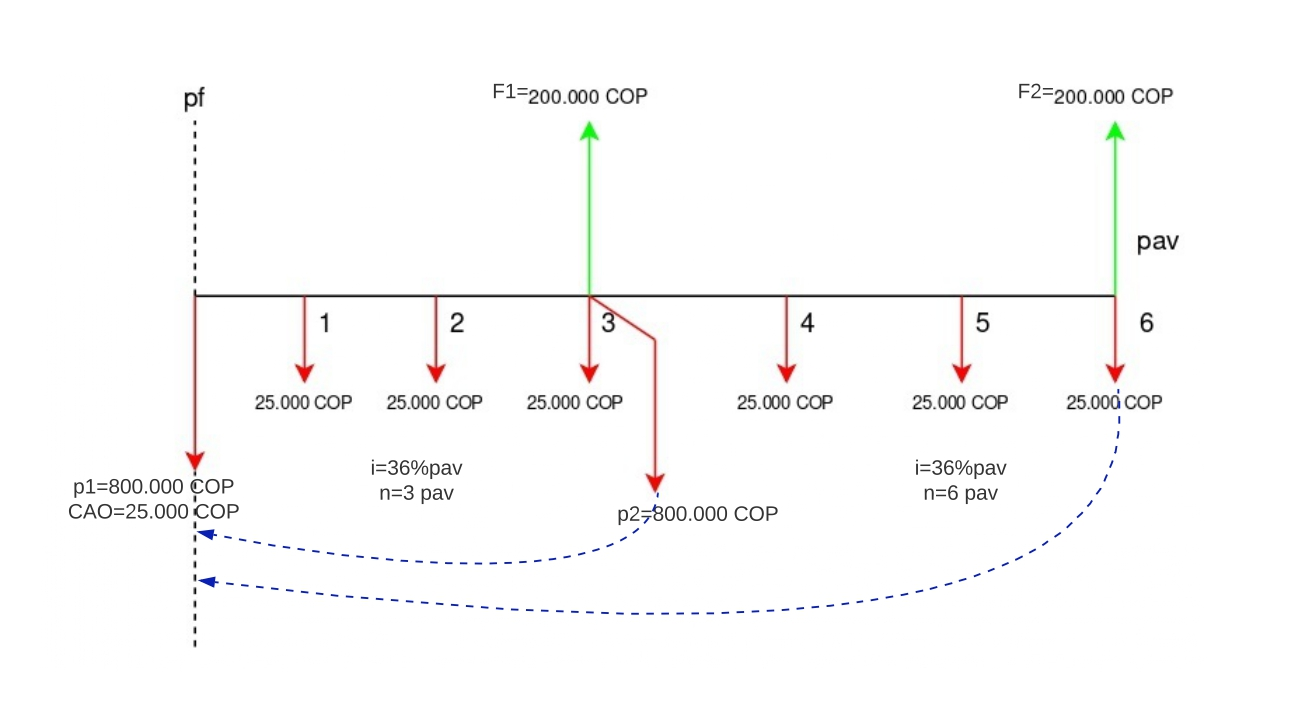
\includegraphics[trim=-5 -5 -5 -5 , scale=1,width=300px, height=250px]{9_Capitulo/ejemplos/4/exportados/ejercicio 4a.png}} 
  \\ 
         \multicolumn{3}{|c|}{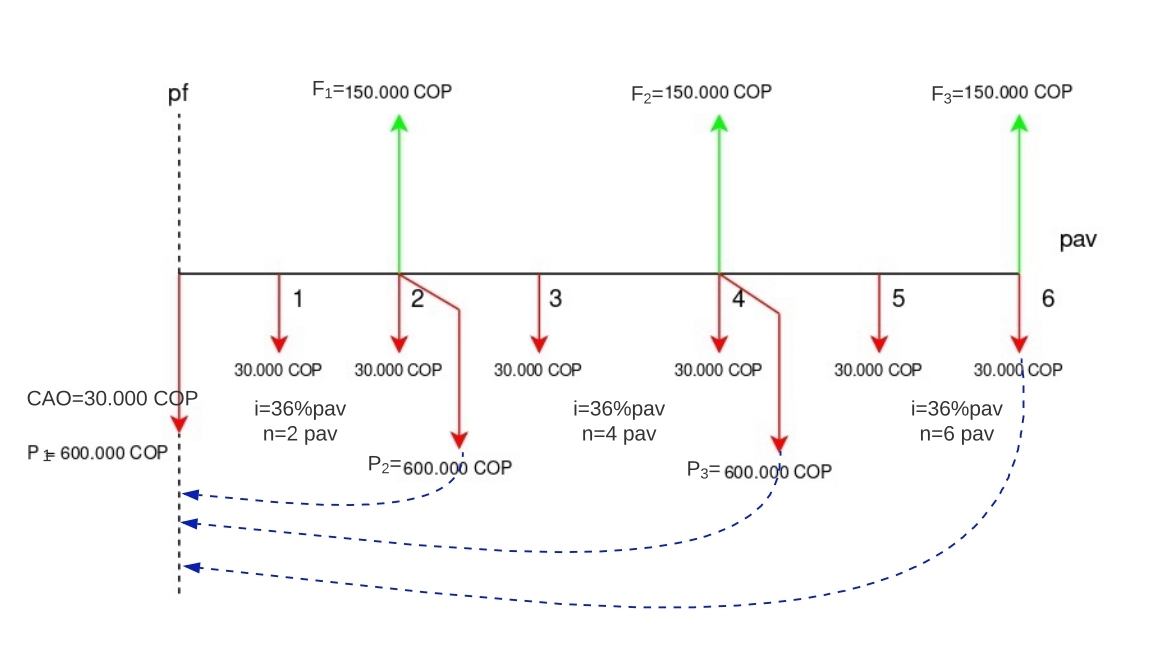
\includegraphics[trim=-5 -5 -5 -5 , scale=1,width=300px, height=250px]{9_Capitulo/ejemplos/4/exportados/ejercicio 4b.png} } \\
         \hline
		%%%%%%%%%%%%% FIN INSERCION DE IMAGEN
		%%%%%FIN FLUJO DE CAJA



		%%%%% INICIO DECLARACION FORMULAS
		%%%%%%%%%%% INICIO TITULO
		\rowcolor[HTML]{FFB183}
		\multicolumn{3}{|c|}{\cellcolor[HTML]{FFB183}\textbf{4. Declaración de fórmulas}}    \\ \hline
		%%%%%%%%%%% FIN TITULO
		%%%%%%%%%%% INICIO MATEMATICAS
		\multicolumn{3}{|c|}{$\sum F_{n}(1+i)^{-n} $\hspace{0.3cm} \textit{Valor presente neto}} \\ \hline
		%%%%%%%%%% FIN MATEMATICAS
		%%%%%% INICIO DESARROLLO MATEMATICO
		\rowcolor[HTML]{FFB183}
		%%%%%%%%%%INICIO TITULO
		\multicolumn{3}{|c|}{\cellcolor[HTML]{FFB183}\textbf{5. Desarrollo matemático}}       \\ \hline
		%%%%%%%%%% FIN TITULO
		%%%%%%%%%% INICIO MATEMATICAS
		\multicolumn{3}{|c|}{$VPN_{A} = -800.000-800.000(1+0.36)^{-3}+200.000(1+0.36)^{-3}$}\\
		\multicolumn{3}{|c|}{$-25.000(1+0.36)^{-6} + 200.000(1+0.36)^{-6}$} \\
		\multicolumn{3}{|c|}{$VPN_{A} = -1.065.338 COP$} \\
		\multicolumn{3}{|c|}{$VPN_{B} = -600.000-30.000(\frac{1-((1+0.36)^{-3})}{0.36})$}\\
		\multicolumn{3}{|c|}{$-450.000 (1+0.36)^{-2}-450.000(1+0.36)^{-4}+150.000  1+0.36)^{-6}$} \\
		\multicolumn{3}{|c|}{$VPN_{B} = -1.021.293 COP$} \\ \hline

		%%%%%%%%%% FIN MATEMATICAS
		%%%%%% FIN DESARROLLO MATEMATICO
		%%%%%% INICIO RESPUESTA
		\rowcolor[HTML]{FFB183}
		%%%%%%%%%%INICIO TITULO
		\multicolumn{3}{|c|}{\cellcolor[HTML]{FFB183}\textbf{6. Respuesta}}   \\ \hline
		%%%%%%%%%% FIN TITULO
		%%%%%%%%%% INICIO RESPUESTA MATEMATICA
		\multicolumn{3}{|c|}{Al hacer la compra de la maquina bajo las condiciones dadas en la alternativa II,}  \\
		\multicolumn{3}{|c|}{la empresa tendrá perdidas, sin embargo, se observa que las perdidas son menores} \\
		\multicolumn{3}{|c|}{que al hacer uso de la Alternativa I, así que se escoge la Alternativa II.}  \\ \hline
		%%%%%%%%%% FIN MATEMATICAS
		%%%%%% FIN RESPUESTA
	\end{longtable}
	%Se crean dos lineas en blanco para que no quede el siguiente texto tan pegado
	%\newline \newline %USARLO SI CREES QUE ES NECESARIO
\end{center}
%%%%%%%%%%%%%%%%%%%%%%%%%%FIN EJERCICIO 4 %%%%%%%%%%%%%%%%%%%%%%%%%%%


\section{ALTERNATIVAS CON VIDA ÚTIL INFINITA}

Cuando las alternativas tienen una vida útil muy grande como en el caso de universidades, organizaciones de caridad, obras civiles tales como represas, puentes, o construcciones con vida útil superior a 40 años, puede considerarse que su vida útil es infinita y que no tienen salvamento y, el error que pueda cometerse viene a ser despreciable (para tasas de interés inferiores a un 10\% deben tomarse mínimo 50 años), para su evaluación se utiliza el método del Costo Capitalizado que representaremos por (C.C.); consiste en hallar un VPN en donde se involucran anualidades infinitas o gradientes infinitos; este método también se utiliza para hallar el punto de equilibrio de dos alternativas.\\
\\
\textbf{Ejemplo 5}\\
Se plantea la construcción de un puente y se han presentado dos proyectos, el primero es un puente colgante a un costo de 850 millones COP y, cada año habrá que darle mantenimiento a la plataforma de asfalto a un costo de 3 millones COP; se estima que las reparaciones serán cada vez mayores y que éstas aumentarán de precio en 2 millones COP cada año, además, cada 5 años habrá que cambiar los cables que sostienen el puente y su costo será de 100 millones COP y, no se prevé que éste valor vaya a cambiar. La segunda alternativa es un puente en concreto a un costo de 900 millones COP y, cada 3 años habrá que reacondicionar las bases a un costo fijo de 25 millones COP; el costo anual de mantenimiento se puede considerar fijo en 5 millones COP. Con una tasa del 25\% pav, determinar la mejor alternativa.\\


%%%%%%%%%%%%%%%%%%% EJERCICIO 5 %%%%%%

%\newpage %USAR SOLO SI EL SOLUCION QUEDA SOLO Y ES NECESARIO BAJARLO A LA SIGUIENTE PAGINA
\textbf{Solución.}\\
%La tabla ira centrada
\begin{center}
	\renewcommand{\arraystretch}{1.5}% Margenes de las celdas
	%Creacion de la cuadricula de 3 columnas \end{flushleft}
	\begin{longtable}[H]{|C{0.3\linewidth}|C{0.3\linewidth}|C{0.3\linewidth}|}
		%Creamos una linea horizontal
		\hline
		%%%%%%%%%% INICIO TITULO
        %%%%% INICIO FLUJO DE CAJA
		\rowcolor[HTML]{FFB183}
		\multicolumn{3}{|c|}{\cellcolor[HTML]{FFB183}\textbf{1. Asignación periodo focal}}   \\ \hline
		\multicolumn{3}{|c|} {$pf : 0 \hspace{0.5em} pav$} \\ \hline
		%%%%%%%%%% FIN TITULO
		%Lo que se hace aqui es mezclar las 3 columnas en una sola
		\multicolumn{3}{|c|}{\cellcolor[HTML]{FFB183}\textbf{2. Declaración de variables}}   \\ \hline
		%%%%%%%%%% FIN TITULO
		%%%%%%%%%% INICIO DE MATEMATICAS
		%Cada & hace referencia al paso de la siguiente columna
		Puente colgante &Puente colgante & i$_{2a}$= ? pav\\ 
		$P_{0}= $ -850.000.000 COP&i$_{1a}$= 25\% pav & i$_{2b}$= ? pav\\
		$P_{1}= $ -3.000.000 COP&n$_{1a}$= 5 pav&$VPN_{A} =$ ? COP\\ 
		$P_{2}= $ -5.000.000 COP&n$_{2a}$= 5 pav&$VPN_{B} =$ ? COP\\ 
        $P_{3}= $ -7.000.000 COP&Puente en concreto\\ 
		$P_{4}= $ -9.000.000 COP&i$_{1b}$= 25 \% pav \\ 
		$P_{5}= $ -111.000.000 COP&n$_{1b}$= 5 pav\\
		Puente en concreto&\\
		$P_{6}= $ -900.000.000 COP&\\
		$P_{7}= $ -5.000.000 COP&\\
		$P_{8}= $ -5.000.000 COP&\\
		$P_{9}= $ -28.000.000 COP&\\
		$P_{10}= $ -5.000.000 COP&\\
		$P_{11}= $ -5.000.000 COP&\\
  \hline
		%%%%%%%%%% FIN DE MATEMATICAS
		%%%%% FIN DECLARACION DE VARIABLES

  		%%%%% INICIO DECLARACION FORMULAS
  
		%%%%%%%%%%% INICIO TITULO
		\rowcolor[HTML]{FFB183}
		\multicolumn{3}{|c|}{\cellcolor[HTML]{FFB183}\textbf{3. Diagrama de flujo de caja}} \\ \hline
		%Mezclamos 3 columnas y ponermos el dibujo
		%%%%%%%%%%%%% INSERCION DE LA IMAGEN
		%Deberan descargar las imagenes respectivas del drive y pegarlas en la carpeta
		%n_capitulo/img/ejemplos/1/capitulo1ejemplo1.pdf  (el /1/ es el numero del ejemplo) 
		\multicolumn{3}{|c|}{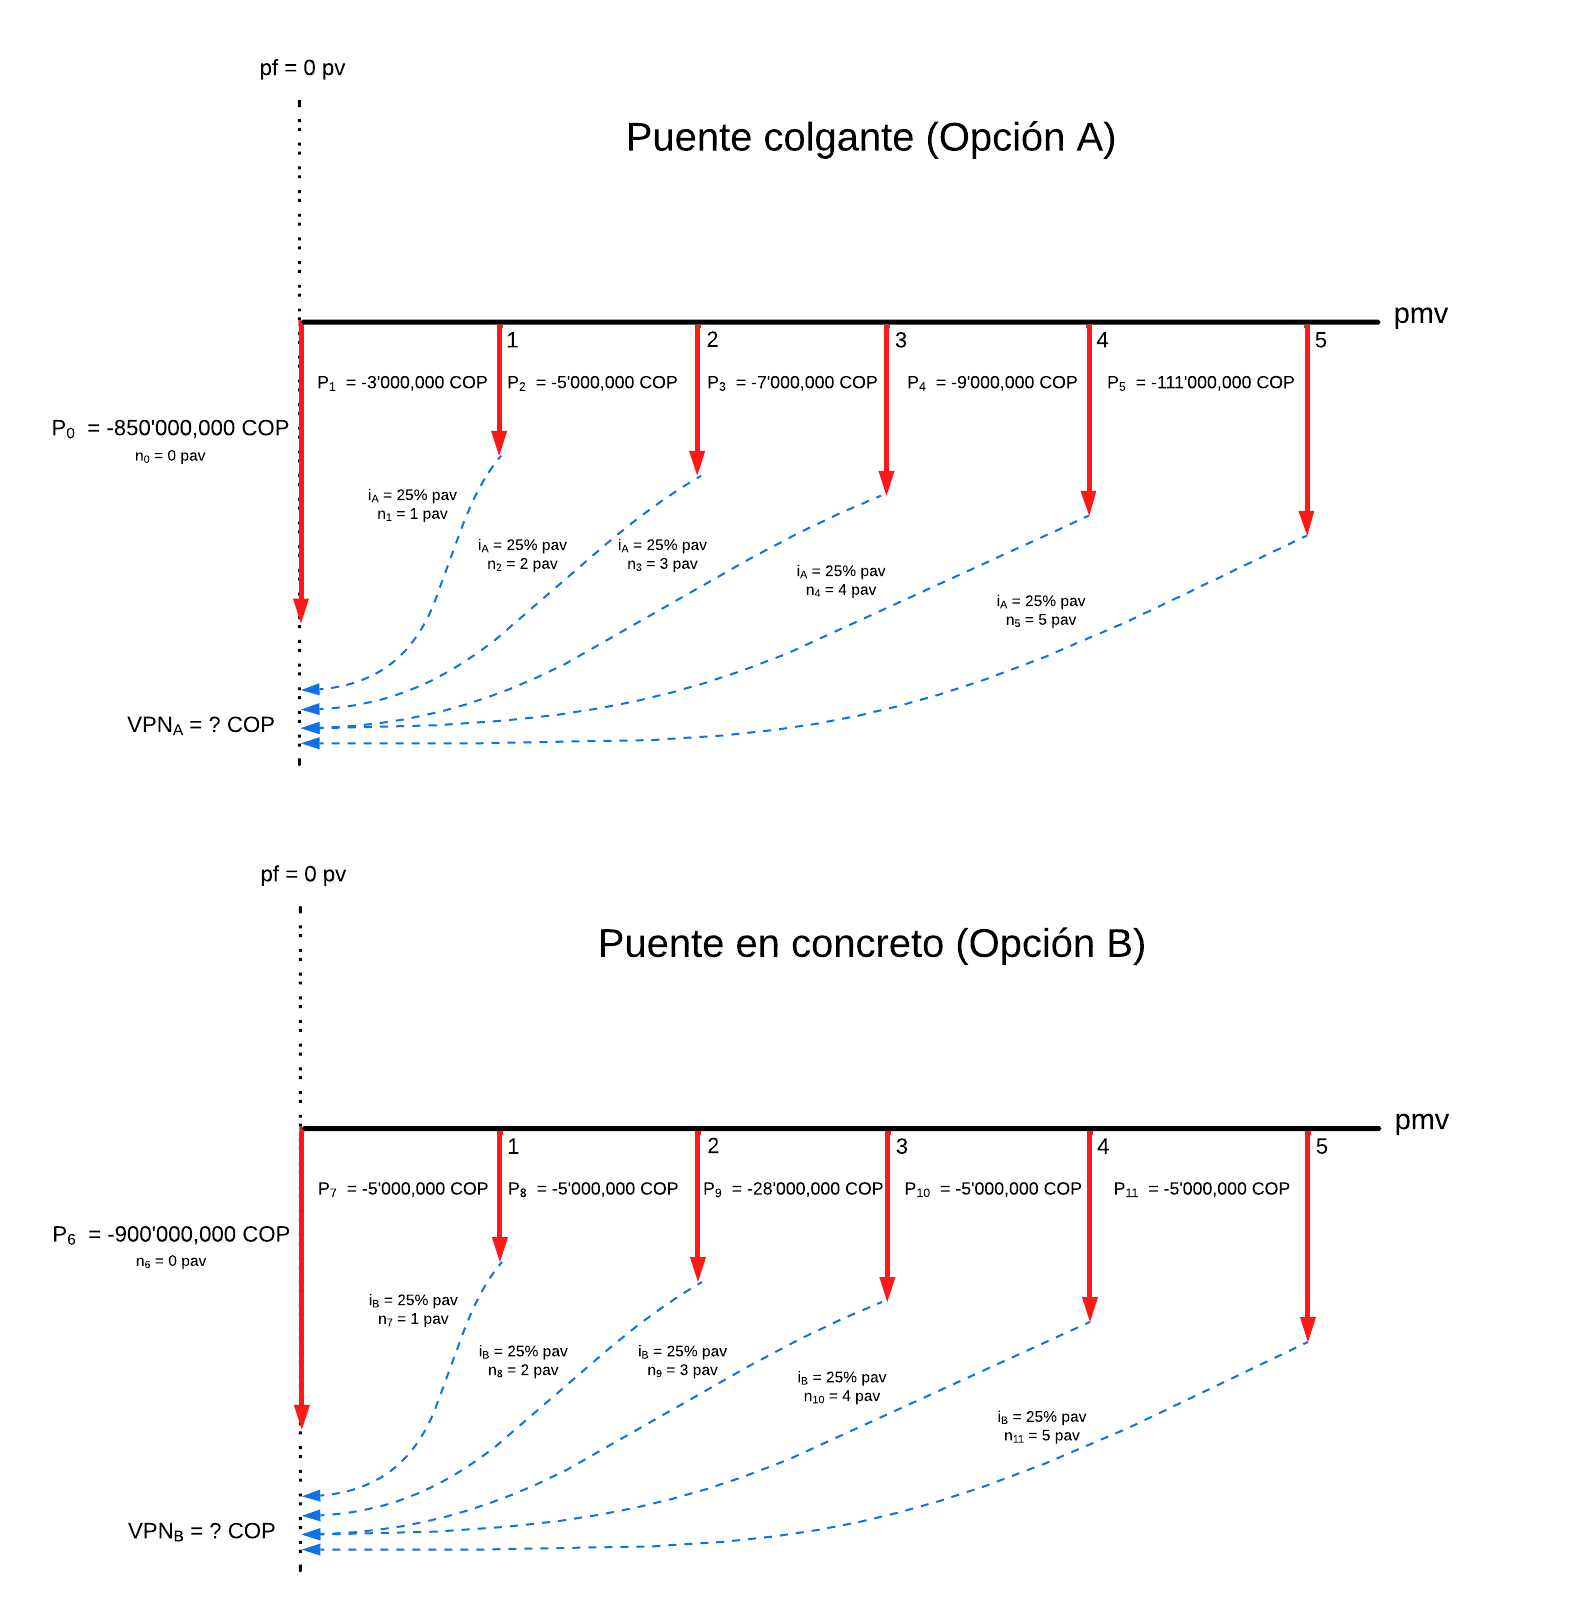
\includegraphics[trim=-5 -5 -5 -5 , scale=2, width=350px, height=480px]{9_Capitulo/ejemplos/6/exportados/Ejemplo5.png}} \\ \hline
		%%%%%%%%%%%%% FIN INSERCION DE IMAGEN
		%%%%%FIN FLUJO DE CAJA



		%%%%% INICIO DECLARACION FORMULAS
		%%%%%%%%%%% INICIO TITULO
		\rowcolor[HTML]{FFB183}
		\multicolumn{3}{|c|}{\cellcolor[HTML]{FFB183}\textbf{4. Declaración de fórmulas}}    \\ \hline
		%%%%%%%%%%% FIN TITULO
		%%%%%%%%%%% INICIO MATEMATICAS
		\multicolumn{3}{|c|}{$\sum F_{n}(1+i)^{-n} $\hspace{0.3cm} \textit{Valor presente neto}} \\
		\multicolumn{3}{|c|}{$(1+i_{1})^{m_{1}} = (1+i_{2})^{m_{2}}$\hspace{0.3cm} \textit{Equivalencia de tasas}} \\ \hline
		%%%%%%%%%% FIN MATEMATICAS
		%%%%%% INICIO DESARROLLO MATEMATICO
		\rowcolor[HTML]{FFB183}
		%%%%%%%%%%INICIO TITULO
		\multicolumn{3}{|c|}{\cellcolor[HTML]{FFB183}\textbf{5. Desarrollo matemático}}  \\ \hline
		%%%%%%%%%% FIN TITULO
		%%%%%%%%%% INICIO MATEMATICAS
		\multicolumn{3}{|c|}{$(1+0.25)^{5} = (1+i_{2})^{1}$ \hspace{0.5cm} $(1+0.25)^{3} = (1+i_{2})^{1}$}\\
		\multicolumn{3}{|c|}{$i_{2} = 205.1757812\% pav$ \hspace{0.5cm} $i_{2} = 95.3125\% pav $} \\
		\multicolumn{3}{|c|}{$VPN_{A} = -850 - \frac{100}{2.051757812} - (\frac{3}{0.25} - \frac{2}{0.0625})$ \hspace{0.5cm}  $VPN_{B} = -900 - \frac{5}{0.25} - \frac{25}{0.953125}$}\\
		\multicolumn{3}{|c|}{$VPN_{A} = - 942.7$ \textit{COP}  \hspace{0.5cm} $VPN_{B} = - 946.23 $ \textit{COP}}\\ \hline

		%%%%%%%%%% FIN MATEMATICAS
		%%%%%% FIN DESARROLLO MATEMATICO
		%%%%%% INICIO RESPUESTA
		\rowcolor[HTML]{FFB183}
		%%%%%%%%%%INICIO TITULO
		\multicolumn{3}{|c|}{\cellcolor[HTML]{FFB183}\textbf{6. Respuesta}}   \\ \hline
		%%%%%%%%%% FIN TITULO
		%%%%%%%%%% INICIO RESPUESTA MATEMATICA
		\multicolumn{3}{|c|}{La mejor elección es construir el puente colgante.}  \\ \hline
		%%%%%%%%%% FIN MATEMATICAS
		%%%%%% FIN RESPUESTA
	\end{longtable}
	%Se crean dos lineas en blanco para que no quede el siguiente texto tan pegado
	%\newline \newline %USARLO SI CREES QUE ES NECESARIO
\end{center}
%%%%%%%%%%%%%%%%%%%%%%%%%%FIN EJERCICIO 5 %%%%%%%%%%%%%%%%%%%%%%%%%%%


\section{EVALUACIÓN DESPUÉS DE IMPUESTO}

Al evaluar un proyecto, es muy importante tener en cuenta los impuestos que deben pagarse. Tomar decisiones sin haber realizado cálculos con impuestos pueden resultar perjudiciales.
Un aspecto que influye notablemente en la liquidación de impuestos es la depreciación, ya que los activos físicos tales como edificios, maquinaria, herramientas, etc; son susceptibles de deterioro debido al uso. Por esta razón, su valor va disminuyendo con el tiempo. Por ello, si en la inversión inicial de un proyecto hay activos físicos, su depreciación afecta a los ingresos, haciendo que se reduzcan los impuestos, causando un aumento en el flujo de caja.(se debe tener claro que la depreciación no es dinero efectivo, sino un asunto puramente contable; pero que en forma indirecta afecta el flujo de caja, ya que reduce la base imponible de los impuestos, lo que puede resultar en una reducción de los impuestos a pagar). Dado que la base para calcular los impuestos son un porcentaje de la base, se halla así:\\

%\paragraph{Base = Ingreso - Costo - Depreciación} //TODO

\textbf{Ejemplo 6}\\
Una industria puede adquirir una máquina a un costo de 6 millones COP, tendrá una vida útil de 5 años y prácticamente no tendrá valor de salvamento, la máquina será depreciada totalmente en 3 años por partes iguales. El estudio de mercados indica que los ingresos del primer año serán aproximadamente de 3 millones COP y aumentarán todos los años un 30\% pav. Por otra parte se estima que el costo de producción del primer año será de 800.000 COP y cada año aumentará en 200.000 COP. Suponiendo una tasa impositiva del 38\% pav, determinar la viabilidad del proyecto con un horizonte de planeación de 5 años y que la tasa del inversionista es del 40\% pav.\\


%%%%%%%%%%%%%%%%%%% EJERCICIO 7 %%%%%%

%\newpage %USAR SOLO SI EL SOLUCION QUEDA SOLO Y ES NECESARIO BAJARLO A LA SIGUIENTE PAGINA
\textbf{Solución.}\\
%La tabla ira centrada
\begin{center}
	\renewcommand{\arraystretch}{1.5}% Margenes de las celdas
	%Creacion de la cuadricula de 3 columnas \end{flushleft}
	\begin{longtable}[H]{|C{0.3\linewidth}|C{0.3\linewidth}|C{0.3\linewidth}|}
		%Creamos una linea horizontal
		\hline
        %%%%% INICIO FLUJO DE CAJA
		\rowcolor[HTML]{FFB183}
		\multicolumn{3}{|c|}{\cellcolor[HTML]{FFB183}\textbf{1. Asignación periodo focal}}   \\ \hline
		\multicolumn{3}{|c|} {$pf : 0 \hspace{0.5em} pav$} \\ \hline
		%%%%%%%%%% FIN TITULO
		%%%%%%%%%% INICIO TITULO
		%Lo que se hace aqui es mezclar las 3 columnas en una sola
		\multicolumn{3}{|c|}{\cellcolor[HTML]{FFB183}\textbf{2. Declaración de variables}}   \\ \hline
		%%%%%%%%%% FIN TITULO
		%%%%%%%%%% INICIO DE MATEMATICAS
		%Cada & hace referencia al paso de la siguiente columna
		$P_{0}= $ -6.000.000 COP & $i_{i}= 30\% pav$ &Decisión final\\
		$F_{1}= $ 3.000.000 COP & $n=1,2,3,4,5 pav$ & \\
		$P_{1}= $ -800.000 COP & $i_{impositiva}= 38\% pav$ & \\
        $F_{2}= $ 3'900.000 COP & $n=1,2,3,4,5 pav$ & \\
        $P{2}= $ -1'000.000 COP & $i_{inversionista}= 40\% pav$ & \\
        $F_{3}= $5'070.000 COP & $i_{imp}= 38\% pav$ & \\
        $P_{3}= $-1'200.000 COP& $n=1,2,3,4,5 pav$& \\
        $F_{4}= $6'591.000 COP&  $n_{1}=1pav $& \\
        $P_{4}= $-1'400.000 COP& $n_{2}=2pav$& \\
        $F_{5}= $8'568.300 COP& $n_{3}=3pav$& \\
        $P_{5}= $-1'600.000 COP& $n_{4}=4pav$& \\
		& $n_{5}=5pav$ & \\
        \hline
        
        
        
        
  
		%%%%%%%%%% FIN DE MATEMATICAS
		%%%%% FIN DECLARACION DE VARIABLES

  		%%%%% INICIO DECLARACION FORMULAS
  
		%%%%%%%%%%% INICIO TITULO
		\rowcolor[HTML]{FFB183}
		\multicolumn{3}{|c|}{\cellcolor[HTML]{FFB183}\textbf{3. Diagrama de flujo de caja}} \\ \hline
		%Mezclamos 3 columnas y ponermos el dibujo
		%%%%%%%%%%%%% INSERCION DE LA IMAGEN
		%Deberan descargar las imagenes respectivas del drive y pegarlas en la carpeta
		%n_capitulo/img/ejemplos/1/capitulo1ejemplo1.pdf  (el /1/ es el numero del ejemplo) 
		\multicolumn{3}{|c|}{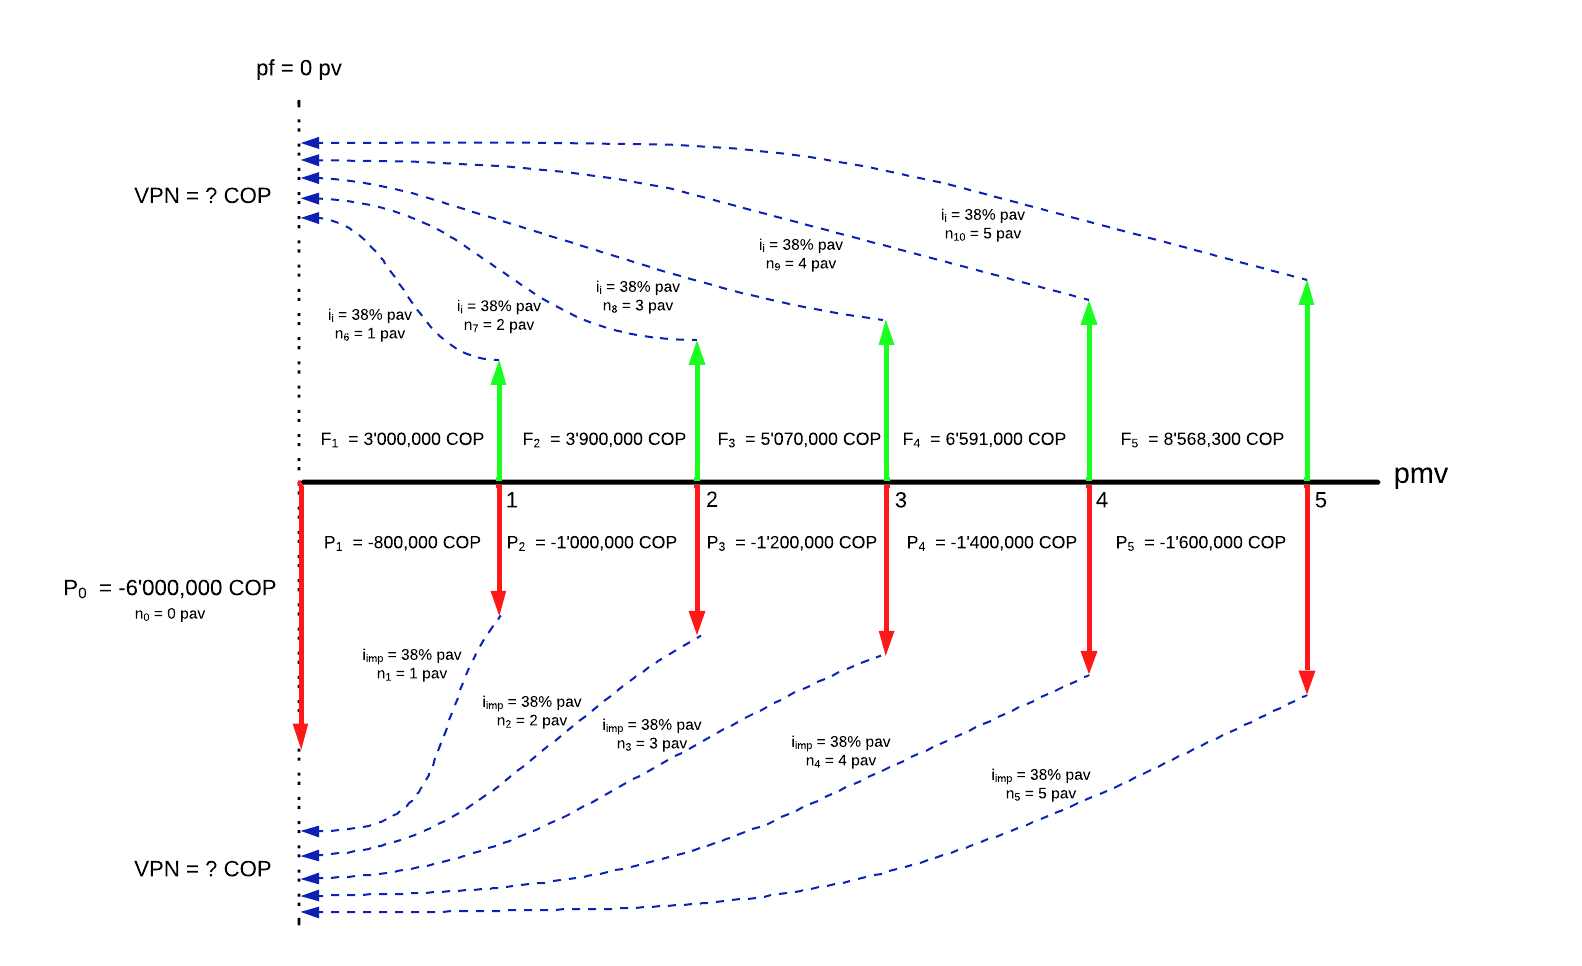
\includegraphics[trim=-5 -5 -5 -5 , scale=1, width=450px, height=300px]{9_Capitulo/ejemplos/7/exportados/Ejemplo6.png}}  \\ \hline
		%%%%%%%%%%%%% FIN INSERCION DE IMAGEN
		%%%%%FIN FLUJO DE CAJA



		%%%%% INICIO DECLARACION FORMULAS
		%%%%%%%%%%% INICIO TITULO
		\rowcolor[HTML]{FFB183}
		\multicolumn{3}{|c|}{\cellcolor[HTML]{FFB183}\textbf{4. Declaración de fórmulas}}    \\ \hline
		%%%%%%%%%%% FIN TITULO
		%%%%%%%%%%% INICIO MATEMATICAS
		\multicolumn{3}{|c|}{$Flujo\_neto\_de\_caja= Ingresos - Cosos - Impuestos$}\\
		\multicolumn{3}{|c|}{$Impuestos=Tasa\_impositiva*Base$}\\
		\multicolumn{3}{|c|}{$Base = Ingreso - Costos - Depreciacion$} \\
		\multicolumn{3}{|c|}{$\sum F_{n}(1+i)^{-n} $\hspace{0.3cm} \textit{Valor presente neto}} \\ \hline
		%%%%%%%%%% FIN MATEMATICAS
		%%%%%% INICIO DESARROLLO MATEMATICO
		\rowcolor[HTML]{FFB183}
		%%%%%%%%%%INICIO TITULO
		\multicolumn{3}{|c|}{\cellcolor[HTML]{FFB183}\textbf{5. Desarrollo matemático}}       \\ \hline
		%%%%%%%%%% FIN TITULO
		%%%%%%%%%% INICIO MATEMATICAS
		
        		\multicolumn{3}{|c|}{
		\resizebox{\textwidth}{!}{%
        			\begin{tabular}{ |c | c |c |c | c |c | c |} 
                    		\hline
                    		PERIODO & INGRESO     & COSTO       & DEPRECIACIÓN & BASE        & IMPUESTO    & FNC         \\
                    		\hline
                    		0       & 6.000.000 COP & 0 COP        & 0 COP         & 0 COP        & 0 COP        & 6.000.000 COP \\
                    		\hline
                    		1       & 3.000000 COP  & 800.000 COP   & 2.000000 COP   & 200.000 COP   & 7.6000 COP    & 2-124.000 COP \\
                    		\hline
                    		2       & 3.900.000 COP & 1.000.000 COP & 2.000.000 COP  & 900.000 COP   & 342.000 COP   & 2.558.000 COP \\
                    		\hline
                    		3       & 5.070.000 COP & 1.200.000 COP & 2.000.000 COP  & 1.870.000 COP & 710.600 COP   & 3.159.400 COP \\
                    		\hline
                    		4       & 6.591.000 COP & 1.400.000 COP & --           & 5.191.000 COP & 1.972.580 COP & 3.218.420 COP \\
                    		\hline
                    		5       & 8.568.300 COP & 1.600.000 COP & --           & 6.968.300 COP & 2.647.954 COP & 4.320.346 COP \\
                    		\hline
            		\end{tabular}}
		}\\ 
	
		\multicolumn{3}{|c|}{$VPN = -6.000.000+2.124.000(1+0.4)^{-1}+2.558.000(1+0.4)^{-2}$}\\
		\multicolumn{3}{|c|}{$+3.159.400(1+0.4)^{-3}+3.218.420(1+0.4)^{-4}+4.320.346(1+0.4)^{-5}$} \\
		\multicolumn{3}{|c|}{$VPN=-385.288 $ COP}\\ \hline

		%%%%%%%%%% FIN MATEMATICAS
		%%%%%% FIN DESARROLLO MATEMATICO
		%%%%%% INICIO RESPUESTA
		\rowcolor[HTML]{FFB183}
		%%%%%%%%%%INICIO TITULO
		\multicolumn{3}{|c|}{\cellcolor[HTML]{FFB183}\textbf{6. Respuesta}}   \\ \hline
		%%%%%%%%%% FIN TITULO
		%%%%%%%%%% INICIO RESPUESTA MATEMATICA
		\multicolumn{3}{|c|}{El proyecto no resulta ser viable, ya que en la ventana de tiempo dado resultaría en pérdidas.}  \\ \hline
		%%%%%%%%%% FIN MATEMATICAS
		%%%%%% FIN RESPUESTA
	\end{longtable}
	%Se crean dos lineas en blanco para que no quede el siguiente texto tan pegado
	%\newline \newline %USARLO SI CREES QUE ES NECESARIO
\end{center}
%%%%%%%%%%%%%%%%%%%%%%%%%%FIN EJERCICIO 1 %%%%%%%%%%%%%%%%%%%%%%%%%%%


\section{FLUJO DE CAJA LIBRE DEL INVERSIONISTA}

Otro procedimiento muy utilizado consiste en presentar el cuadro utilizando el formato de Estado de Resultados. Para ello debemos utilizar las siguientes fórmulas, en donde relacionamos las principales cuentas:\\

\begin{enumerate}
	\item Utilidad bruta = Ingresos - Egresos
	      \begin{itemize}
		      \item En ingresos figuran ventas.
		      \item En egresos figuran todos los costos directos de producción, tales como: materia prima, honorarios, salarios, depreciaciones de máquinas y equipos utilizados directamente en la producción, gastos generales de la planta como energía, agua, etc.\\
	      \end{itemize}
	\item Utilidad operativa = Utilidad bruta - Gastos operacionales.
	      \begin{itemize}
		      \item La cuenta de gastos operacionales incluyen todos los gastos en que se incurren indirectamente en la producción tales como: Depreciación de muebles y enseres utilizados en la administración, gastos administrativos, propaganda, etc.\\
	      \end{itemize}
	\item Utilidad antes de impuestos = Utilidad operativa + Otros ingresos - Otros egresos
	      \begin{itemize}
		      \item En la cuenta de otros ingresos figuran los intereses por activos financieros, tales como CDTs.
		      \item En la cuenta de otros egresos figuran los intereses pagados por préstamos, venta de activos, salvamentos, etc.\\
	      \end{itemize}
	\item Utilidad después de impuestos = Utilidad antes de impuestos - Impuestos\\
	      
	\item Flujo neto de caja para el inversionista = Utilidad después de impuestos - Inversiones - Amortizaciones + Depreciaciones.
\end{enumerate}

\section{FLUJO DE CAJA LIBRE DEL PROYECTO}

Este flujo consiste en suponer que todos los recursos invertidos en el proyecto son recursos propios, es decir, asumir que no existe financiación. En consecuencia, no se toman en cuenta ni los intereses ni las cuotas de amortización. En este caso deberán utilizarse las siguientes fórmulas:\\

\begin{enumerate}
	\item Impuestos = (Utilidad antes de impuestos + Intereses) x Tasa impositiva\\
	\item Flujo de caja libre del proyecto = Utilidad antes de impuestos + Intereses + Depreciaciones + Amortizaciones - Impuestos - Inversiones.\\
\end{enumerate}
Este sistema solo se puede utilizar cuando no hay financiación.\\

El VAN de un proyecto aplicado al flujo de caja del inversionista puede indicar si el proyecto es bueno, sin embargo, no necesariamente debe ser aceptado; pues si se evalúa con el flujo de caja libre del proyecto, puede que no sea aceptado. Esto puede ocurrir cuando el proyecto es apalancado financieramente y que la tasa de financiación sea inferior a la TIO, pero si se le retira el apalancamiento el proyecto se vuelve deficiente.\\

Cuando se utiliza el financiamiento se corre el riesgo de trabajar con proyectos indeseables, este riesgo se elimina si lo evaluamos retirando la financiación, es decir, evaluando con el flujo libre del proyecto.\\

Cuando se evalúa un proyecto con el flujo de caja, el proyecto es más difícil de ser aceptado, porque este es más exigente que el flujo de caja del inversionista. De lo anterior se concluye que la evaluación con el flujo de caja libre del proyecto, minimiza el riesgo de pérdida cuando las variables proyectadas cambian desfavorablemente durante la ejecución del mismo.\\\\
\\
\textbf{Ejemplo 7}\\
Un proyecto necesita adquirir una máquina a un costo de 8 millones COP, de los cuales 3 millones COP serán financiados por un banco que cobra un interés del 20\% pav. La máquina será depreciada en línea recta en 3 años. Los ingresos anuales se estiman en 7 millones COP y los egresos anuales en 1 millón COP. Suponiendo que los inversionistas esperan ganarse un 40\% pav. Con un horizonte de planeación de 3 años y una tasa impositiva del 35\% pav. Determinar la viabilidad financiera del proyecto. Usando el flujo de caja para el accionista (FCLA) y usando el flujo de caja libre del proyecto (FCLP).\\\\
Comparar y analizar los resultados.


%%%%%%%%%%%%%%%%%%% EJERCICIO 8 %%%%%%

%\newpage %USAR SOLO SI EL SOLUCION QUEDA SOLO Y ES NECESARIO BAJARLO A LA SIGUIENTE PAGINA
\textbf{Solución.}\\
%La tabla ira centrada
\begin{center}
	\renewcommand{\arraystretch}{1.5}% Margenes de las celdas
	%Creacion de la cuadricula de 3 columnas \end{flushleft}
	\begin{longtable}[H]{|C{0.3\linewidth}|C{0.3\linewidth}|C{0.3\linewidth}|}
		%Creamos una linea horizontal
		\hline
        %%%%% INICIO FLUJO DE CAJA
		\rowcolor[HTML]{FFB183}
		\multicolumn{3}{|c|}{\cellcolor[HTML]{FFB183}\textbf{1. Asignación periodo focal}}   \\ \hline
		\multicolumn{3}{|c|} {$pf : 0 \hspace{0.5em} pav$} \\ \hline
		%%%%%%%%%% FIN TITULO
		%%%%%%%%%% INICIO TITULO
		%Lo que se hace aqui es mezclar las 3 columnas en una sola
		\multicolumn{3}{|c|}{\cellcolor[HTML]{FFB183}\textbf{2. Declaración de variables}}   \\ \hline
		%%%%%%%%%% FIN TITULO
		%%%%%%%%%% INICIO DE MATEMATICAS
		%Cada & hace referencia al paso de la siguiente columna
		$F_{1}= $ 7.000.000 COP & $n=3\text{ pav}$ &Decisión final   \\
		$P_{1}= $ 3.000.000 COP & $i_{inver}= 40\%\text{ pav}$ & \\
		$F_{2}= $ 1.000.000 COP& $i_{impositiva}=35\%\text{ pav}$ & \\ 
		P$_{2}= $ 1.000.000 COP& $i=20\% \text{ pav}$& \\
		& n$_{2}$ = 3\text{ pav} & \\
		\hline
		%%%%%%%%%% FIN DE MATEMATICAS
		%%%%% FIN DECLARACION DE VARIABLES

  		%%%%% INICIO DECLARACION FORMULAS
  
		%%%%%%%%%%% INICIO TITULO
		\rowcolor[HTML]{FFB183}
		\multicolumn{3}{|c|}{\cellcolor[HTML]{FFB183}\textbf{3. Diagrama de flujo de caja}} \\ \hline
		%Mezclamos 3 columnas y ponermos el dibujo
		%%%%%%%%%%%%% INSERCION DE LA IMAGEN
		%Deberan descargar las imagenes respectivas del drive y pegarlas en la carpeta
		%n_capitulo/img/ejemplos/1/capitulo1ejemplo1.pdf  (el /1/ es el numero del ejemplo) 
		\multicolumn{3}{|c|}{ 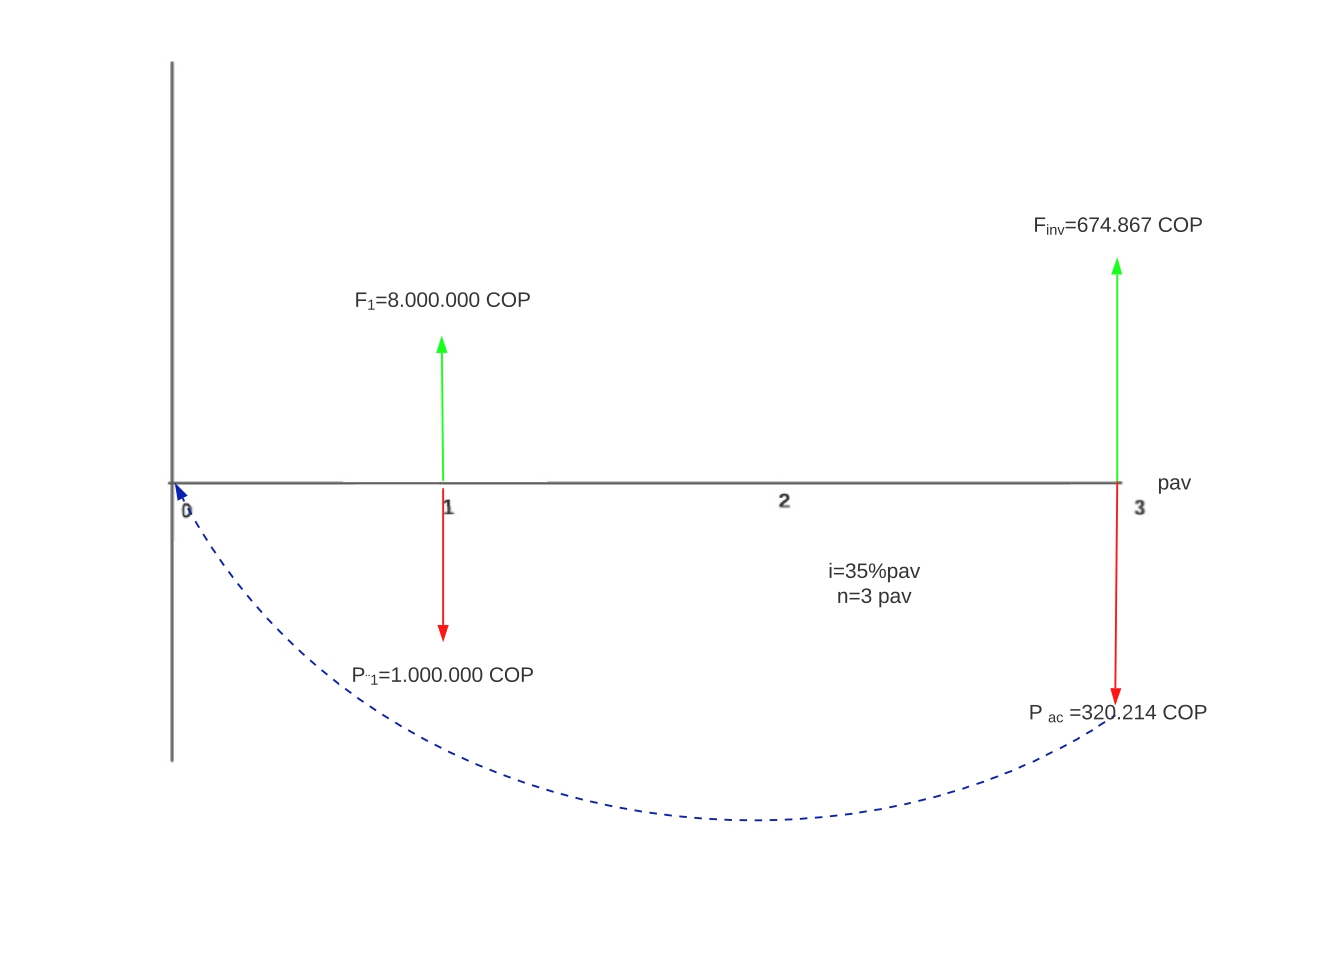
\includegraphics[trim=-5 -5 -5 -5 , scale=1, width=300px, height=250px]{9_Capitulo/ejemplos/8/exportados/Cap9Ejercicio8.png} }   \\ \hline
		%%%%%%%%%%%%% FIN INSERCION DE IMAGEN
		%%%%%FIN FLUJO DE CAJA



		%%%%% INICIO DECLARACION FORMULAS
		%%%%%%%%%%% INICIO TITULO
		\rowcolor[HTML]{FFB183}
		\multicolumn{3}{|c|}{\cellcolor[HTML]{FFB183}\textbf{4. Declaración de fórmulas}}    \\ \hline
		%%%%%%%%%%% FIN TITULO
		%%%%%%%%%%% INICIO MATEMATICAS
		\multicolumn{3}{|c|}{$Flujo\_de\_caja\_libre\_del\_proyecto= utilidades\_antes\_de\_impuestos$}\\
		\multicolumn{3}{|c|}{$+ intereses+ depreciaciones + amortizaciones - impuestos - inversiones$}\\
		\multicolumn{3}{|c|}{$impuestos=(utilidades\_antes\_de\_impuestos+intereses)*tasa\_impositiva$} \\ \hline
		%%%%%%%%%% FIN MATEMATICAS
		%%%%%% INICIO DESARROLLO MATEMATICO
		\rowcolor[HTML]{FFB183}
		%%%%%%%%%%INICIO TITULO
		\multicolumn{3}{|c|}{\cellcolor[HTML]{FFB183}\textbf{5. Desarrollo matemático}}       \\ \hline
		%%%%%%%%%% FIN TITULO
		%%%%%%%%%% INICIO MATEMATICAS
		\multicolumn{3}{|c|}{}\\ 
		\multicolumn{3}{|c|}{\textbf{1. Usando el flujo de caja para el accionista (FCLA):}}\\ 
        		\multicolumn{3}{|c|}{
		\resizebox{\textwidth}{!}{%
        			\begin{tabular}{|c |c |c |c |c |}                                                             \hline
                            	AÑO                         & 0            & 1            & 2            & 3            \\ \hline
                            	INGRESOS                    & --           & 7.000.000 COP  & 7.000.000 COP  &  7.000.000 COP \\ \hline
                            	EGRESOS                     & --           & 1.000.000 COP  & 1.000.000 COP  & 1.000.000 COP  \\\hline
                            	DEPRECIACIÓN                & --           & 2.666.667 COP  & 2.666.667 COP & 2.666.666 COP  \\ \hline
                            	UTILIDAD BRUTA              & --           &  3.333.333 COP & 3.333.333 COP  &  3.333.334 COP \\\hline
                            	GASTOS OPERACIONALES        & --           & 0 COP          & 0 COP          & 0 COP          \\\hline
                            	UTILIDAD OPERACIONAL        & --           &  3.333.333 COP & 3.333.333 COP  &  3.333.334 COP \\\hline
                            	GASTOS FINANCIEROS          & --           & 600.000 COP   & 435.162 COP    &  237.363 COP   \\\hline
                            	UTILIDAD ANTES DE IMPUESTAS & --           &  2.733.333 COP & 2.898.168 COP  & 3.095.971 COP  \\\hline
                            	INVERSIONES                 & 5.000.000 COP  & --           & --           & \ --         \\\hline
                            	AMORTIZACIÓN                & --           &  824.176 COP   & 989.011 COP    &  1.186.813 COP \\\hline
                            	DEPRECIACIONES              & --           &  2.666.667 COP & 2.666.667 COP  &  2.666.666 COP \\\hline
                            	FNC PARA INVERSIONISTAS     & -5.000.000 COP &  3.619.157 COP & 3.561.465 COP  &  3.492.234 COP \\\hline
                            	TIO                         & 40\%         & VA           &  674.867 COP       &           \\\hline
                        \end{tabular}}
		}\\ 
		\multicolumn{3}{|c|}{}\\
		\multicolumn{3}{|c|}{\textbf{2. Usando el flujo de caja libre del proyecto (FCLP):}}\\
        		\multicolumn{3}{|c|}{
		\resizebox{\textwidth}{!}{%
        			\begin{tabular}{ |c | c| c| c| c|}
                    		\hline
                    		AÑO                         & 0  & 1            & 2           & 3           \\\hline
                    		UTILIDAD ANTES DE IMPUESTAS & -- &  2.733.333  COP & 2.898.168  COP & 3.095.971 COP \\\hline
                    		+ INTERESES (20\%)          & -- & 600.000 COP    & 435.165 COP   & 237.363 COP   \\  \hline
                    		IMPUESTOS                   & -- & 1.166.667 COP  & 1.166.667 COP & 1.166.667 COP \\  \hline
                    	\end{tabular}}
		}\\
		\multicolumn{3}{|c|}{}\\ 
		\multicolumn{3}{|c|}{\textbf{FLUJO DE CAJA LIBRE PROYECTO:}}\\
        		\multicolumn{3}{|c|}{
		\resizebox{\textwidth}{!}{%
        			\begin{tabular}{ |c | c| c| c| c|}
                    		\hline
                    		AÑO                         & 0            & 1            & 2           & 3                \\\hline
                    		UTILIDAD ANTES DE IMPUESTAS & --           & 2.733.333 COP & 2.898.168 COP & 3.095.971 COP      \\\hline
                    		INTERESES                   & --           & 600.000 COP    & 435.165 COP   & 237.363 COP        \\  \hline
                    		IMPUESTOS                   & --           & 1.166.667 COP  & 1.166.667 COP & 1.166.667 COP      \\  \hline
                    		DEPRECIACIONES              & --           &  2.666.667 COP & 2.666.667 COP & 2.666.666 COP      \\\hline
                    		INVERSIONES                 & -8.000.000 COP &  4.833.333 COP & 4.833.333 COP & 4.833.333 COP      \\\hline
                    		F.C LIBRE DEL PROYECTO      & -320.214 COP  & TIO =  40\%  & TIO =  40\% & VAN = -320.214 COP \\\hline
                    	\end{tabular}}
		}\\ 
		\multicolumn{3}{|c|}{}\\ \hline

		%%%%%%%%%% FIN MATEMATICAS
		%%%%%% FIN DESARROLLO MATEMATICO
		%%%%%% INICIO RESPUESTA
		\rowcolor[HTML]{FFB183}
		%%%%%%%%%%INICIO TITULO
		\multicolumn{3}{|c|}{\cellcolor[HTML]{FFB183}\textbf{6. Respuesta}}   \\ \hline
		%%%%%%%%%% FIN TITULO
		%%%%%%%%%% INICIO RESPUESTA MATEMATICA
		\multicolumn{3}{|c|}{En conclusión el proyecto no es bueno, debido a que si bien el flujo de caja del inversionista}  \\ 
		\multicolumn{3}{|c|}{es de 674.867 COP, el del accionista marca perdidas con un valor de 320.214 COP.}\\
		\multicolumn{3}{|c|}{Por lo tanto, no satisface a las dos partes.}\\ \hline
		%%%%%%%%%% FIN MATEMATICAS
		%%%%%% FIN RESPUESTA
	\end{longtable}
	%Se crean dos lineas en blanco para que no quede el siguiente texto tan pegado
	%\newline \newline %USARLO SI CREES QUE ES NECESARIO
\end{center}
%%%%%%%%%%%%%%%%%%%%%%%%%%FIN EJERCICIO 1 %%%%%%%%%%%%%%%%%%%%%%%%%%%

